\documentclass[a4paper, 10pt, font=plain]{abnt}
\usepackage[utf8]{inputenc}
\usepackage[brazil]{babel}
\usepackage{graphicx}
\usepackage[alf]{abntcite}

\begin{document}
\title{Resumo do livro Agile Coaching}
\author{Hugo Lopes Tavares}
\date{\today}

\maketitle

\part{Coaching Basics}

\chapter{Começando a Jornada}
A missão de um Agile Coach é guiar equipes pra que elas produzam software de qualidade usando métodos ágeis. ``O que um Agile Coach faz?'', ``Como eu faço isso?'', são perguntas que provavelmente desaparecerão ao ler o livro Agile Coaching e esse capítulo cobrirá os tópicos básicos.

\section{O que um Agile Coach faz?}
Seu objetivo é guiar equipes para que elas consigam pensar por si próprias, ao invés de depender de você para ditar leis. Os membros da equipe precisam trocar a maneira como eles pensam e trabalham pra que a implantação de ágil dê certo. Como um agile coach o seu trabalho é guiá-los até que eles encontrem seu próprio caminho.

  \begin{figure}[h]
    \centering
    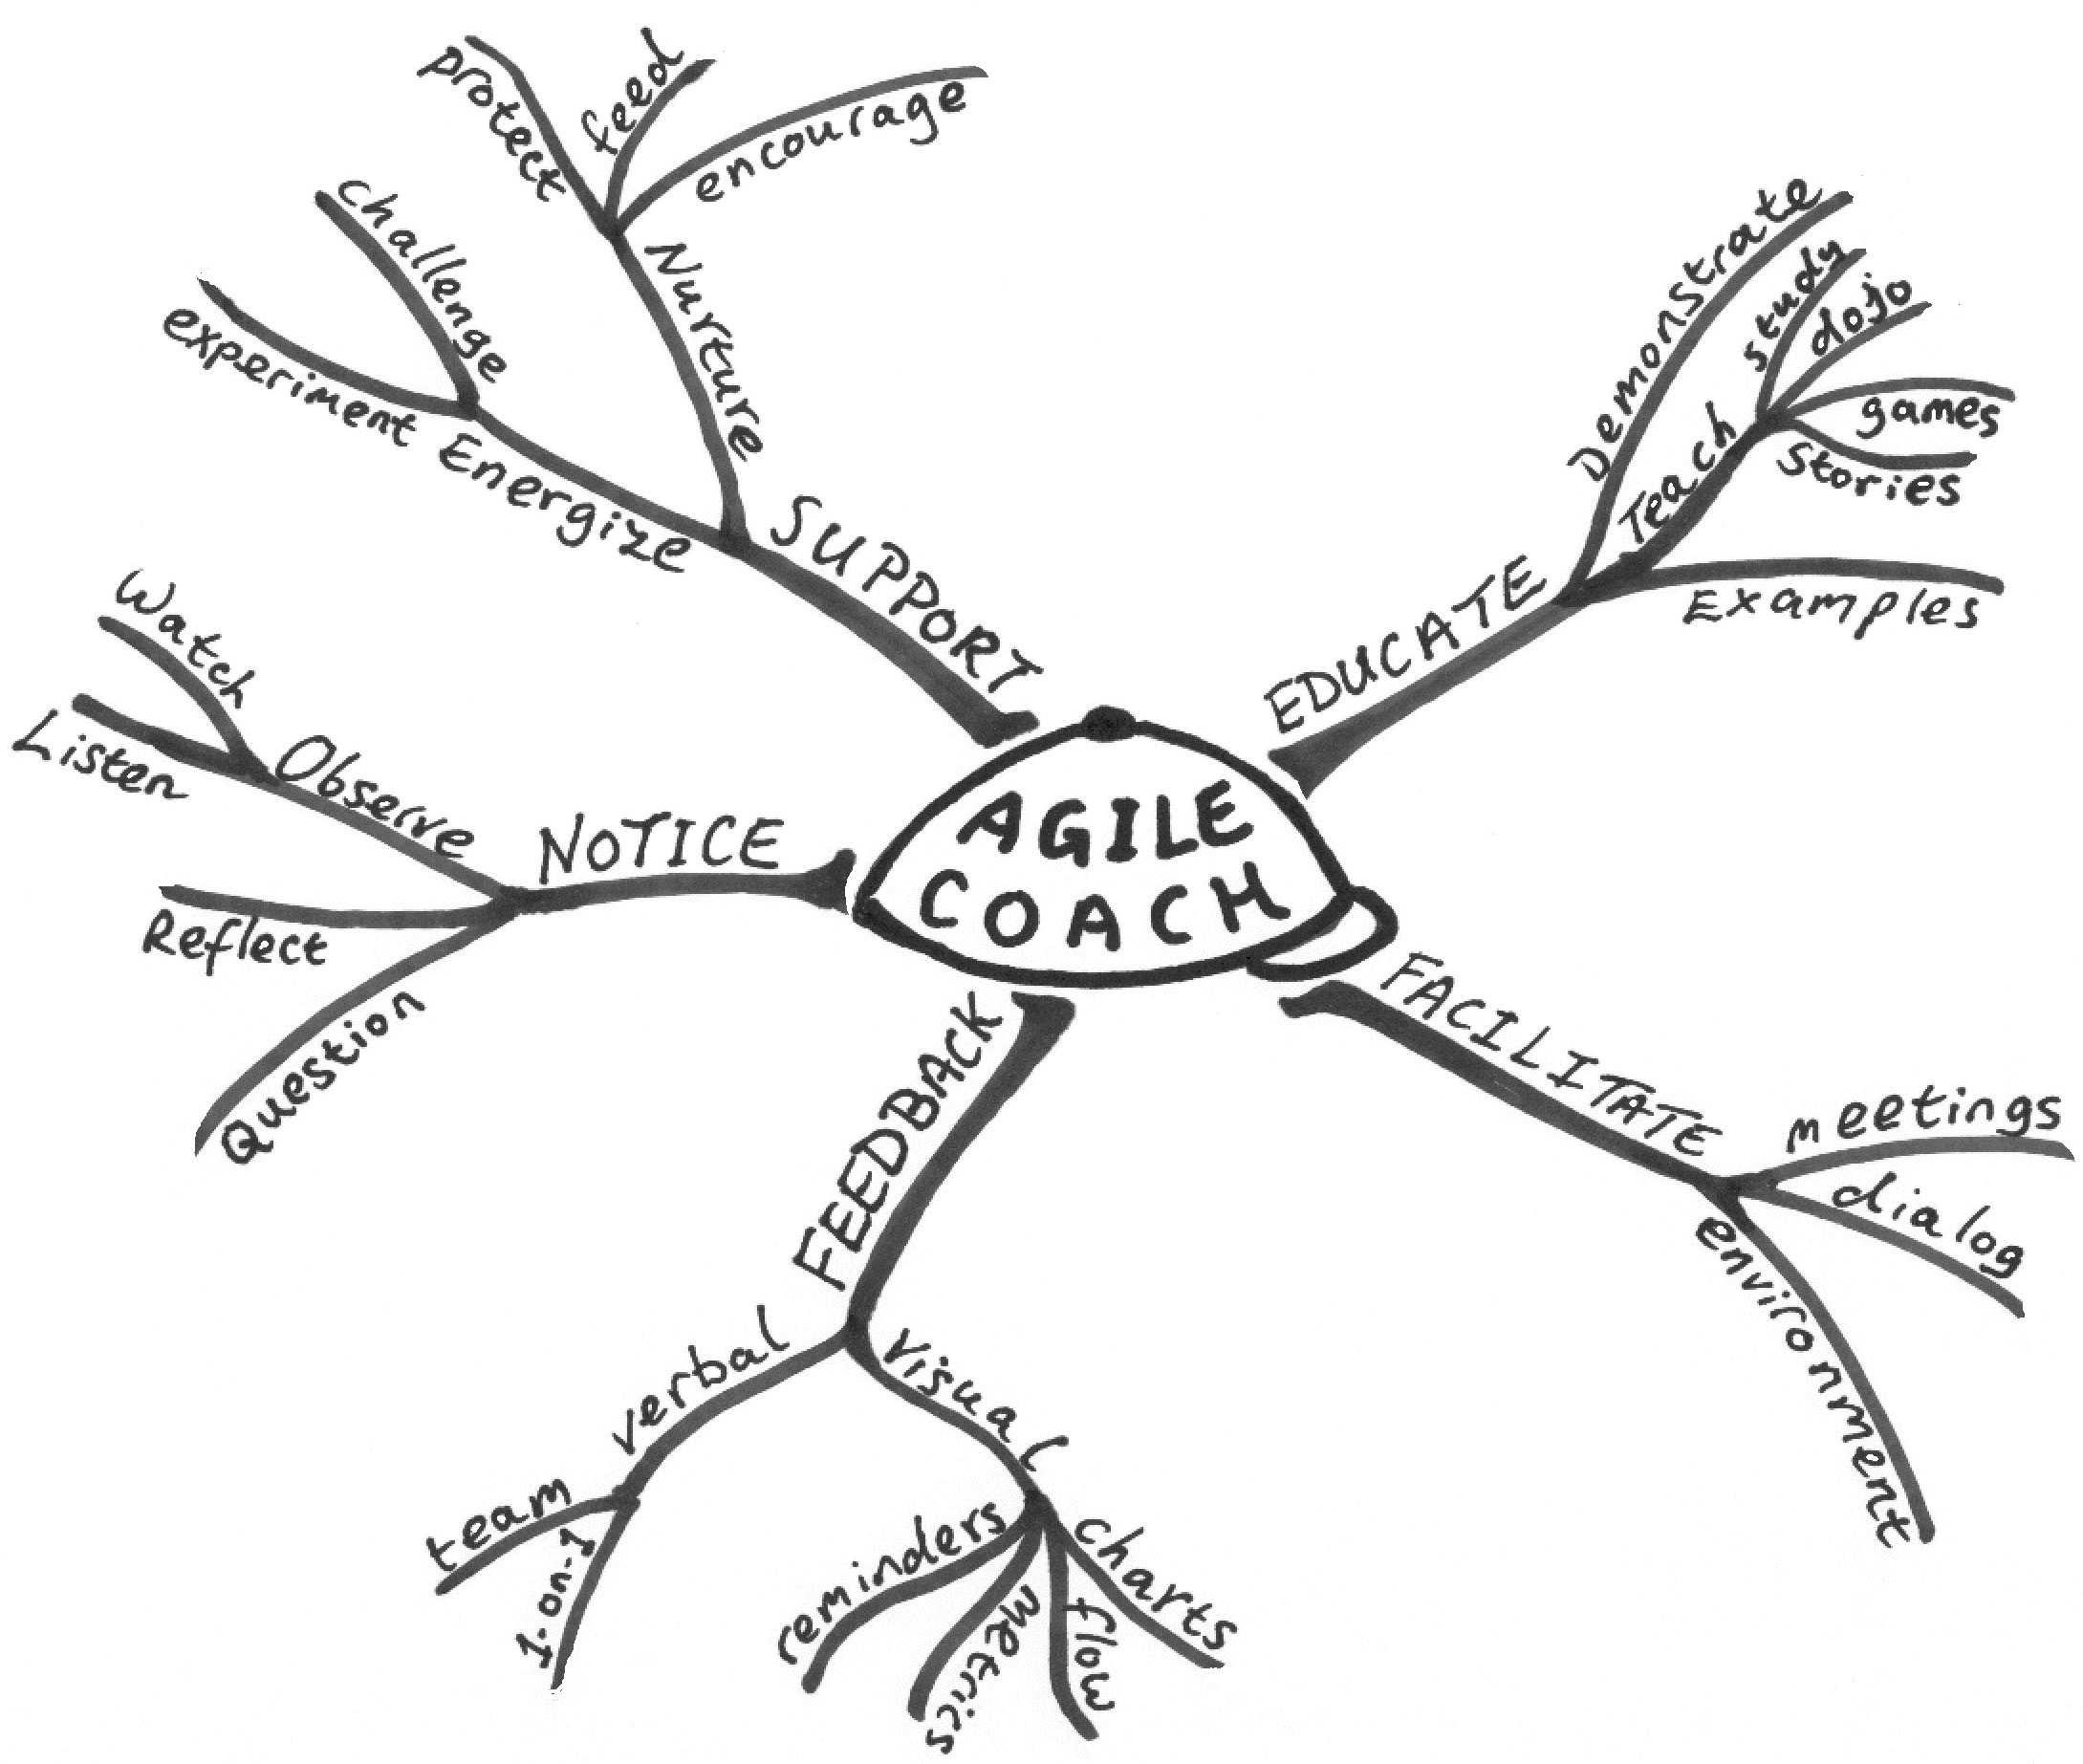
\includegraphics[width=8cm]{mind_map_capitulo1}
    \caption{Mapa mental sobre as tarefas de um agile coach}
  \end{figure}



\section{Desenvolvendo a Atitude de Coach}
O essencial para quem quer se tornar coach é a atitude. Você precisa acreditar que o processo de mudança é possível antes de acontecer e estar sempre aberto a novas idéias.
Algumas das habilidades que todo agile coach precisa desenvolver estão nas próximas seções.

\subsection{Seja um Exemplo}
Todo coach deve dar o exemplo para a equipe. O coach tem que seguir fielmente o que prega, para que possa passar confiança pra equipe. Quando você faz o que fala, as pessoas veêm que podem confiar em você.

\subsection{Mantenha o Equilíbrio}
É normal que as mudanças introduzidas por você causem na equipe uma reação que nem sempre é a esperada. Nunca leve as críticas pro lado pessoal, mantenha-se positivo e firme no papel de coach.

\subsection{Defina um Passo Sustentável}
Não espere perfeição nos primeiros passos de nenhuma equipe, mudanças levam tempo. Paciência é uma das qualidades de um coach.

Se uma equipe está devagar demais pra aplicar o que você tem sugerido, tente achar a causa disso. Será que você está indo rápido demais? Será que não é uma boa hora pra começar?
Seja persistente, afinal, você quer ver resultados. Tente achar novas maneiras pra ajudar a equipe a ver que as mudanças pra Agile são importantes.

\subsection{Pense no seu Vocabulário}
Um coach deve observar o seu vocábulário, pois ele precisa ser claro e você tem que passar idéias facilmente.
Algumas palavras devem ser trocadas para que você possa parecer parte da equipe. Ao invés de dizer ``Você precisa consertar o build'', diga ``Nós precisamos consertar o build''. A diferença é bem pequena, mas os efeitos que essas mudanças causam são importantes, pois mostram que você está do lado da equipe.

Evite criar categorias como ``os desenvolvedores'', ``a gerência'', pois tais categorias criam barreiras na comunicação.

\section{Aprenda com Suas Experiências}
Quando as coisas não sairem como o esperado, não adianta entrar em pânico, pois você deve aprender com os seus erros. Talvez na próxima vez que se deparar com a mesma situção, você deva tentar uma abordagem diferente.

Você não deve ficar encima da equipe o tempo inteiro. Tire um tempo pra refrescar as idéias e se atualizar no que tem acontecido nas comunidades ágeis e fora da empresa. Leia livros, blogs, ouça podcasts e conecte-se com pessoas que tenham os mesmos interesses que você.


\section{Estando Pronto pra Fazer Coach}
Assim como um treinador de esportes, você tem que saber como o jogo funciona. Quando você tiver mais experiência com Agile, poderá usar exemplos reais pra ilustrar seus pontos pra equipes.

Pratique e aprenda como Agile funciona, aprenda a responder perguntas inesperadas. Encontre alguém que queira ouvir e não saiba do que Agile se trata, para que você possa praticar explicações sobre Agile.

Antes de trabalhar com alguma equipe entenda melhor o seu papel. Quais benefícios você traz pra uma equipe? O que a equipe e a gerência esperam de você? Reflita sobre essas questões pra facilitar sua apresentação pra equipe.


\section{Prepare-se pra ser Apresentado}
Começar com o pé direito é muito importante. Você tem que ser apresentado pra equipe, mas trate de fazer isso da melhor maneira. Certifique-se que as pessoas entendam seu papel na equipe.

Ter uma boa apresentação faz com que a equipe tenha credibilidade no seu trabalho. Você precisa fazer com que eles entendam o que você está pronto a oferecer e como você pode dar suporte pra equipe.

A apresentação pode ser feita por várias pessoas dependendo da situação. Você pode ser apresentado pelo empregador, caso você esteja sendo contrato como um coach externo. O empregador pode citar suas qualidades e o que você tem feito como coach ou desenvolvedor.
Caso você já faça parte de uma empresa e tenha sido solicitado pra trabalhar como coach num projeto piloto ou algo parecido, faça com que um gerente que tenha autoridade o suficiente, te apresente pra equipe e mostre a confiança que a empresa tem em você nesse papel. Porém, caso você simplesmente queira disseminar as idéias ágeis, porque você acredita nessa filosofia e tem autoridade pra estender seu papel pra ser um agile coach, não há necessidades de ninguém te apresentar -- as pessoas já te conhecem. Junte os membros da equipe e mostre a eles o seu novo papel e responda às perguntas iniciais que aparecerem sobre o movimento ágil.

Após as apresentações gaste um pouco de tempo pra ver como a equipe trabalha -- observe de perto. Tente se camuflar como um camaleão para que você consiga pegar os melhores momentos da equipe.

A equipe precisa ter confiança em você antes de começar a seguir suas idéias. Talvez uma sesão pra explicar sobre Agile, algum XP game ou um coding dojo, facilite a introdução dessas novas idéias.



\section{Como começar a fazer coaching}
    \begin{figure}[h]
        \centering
        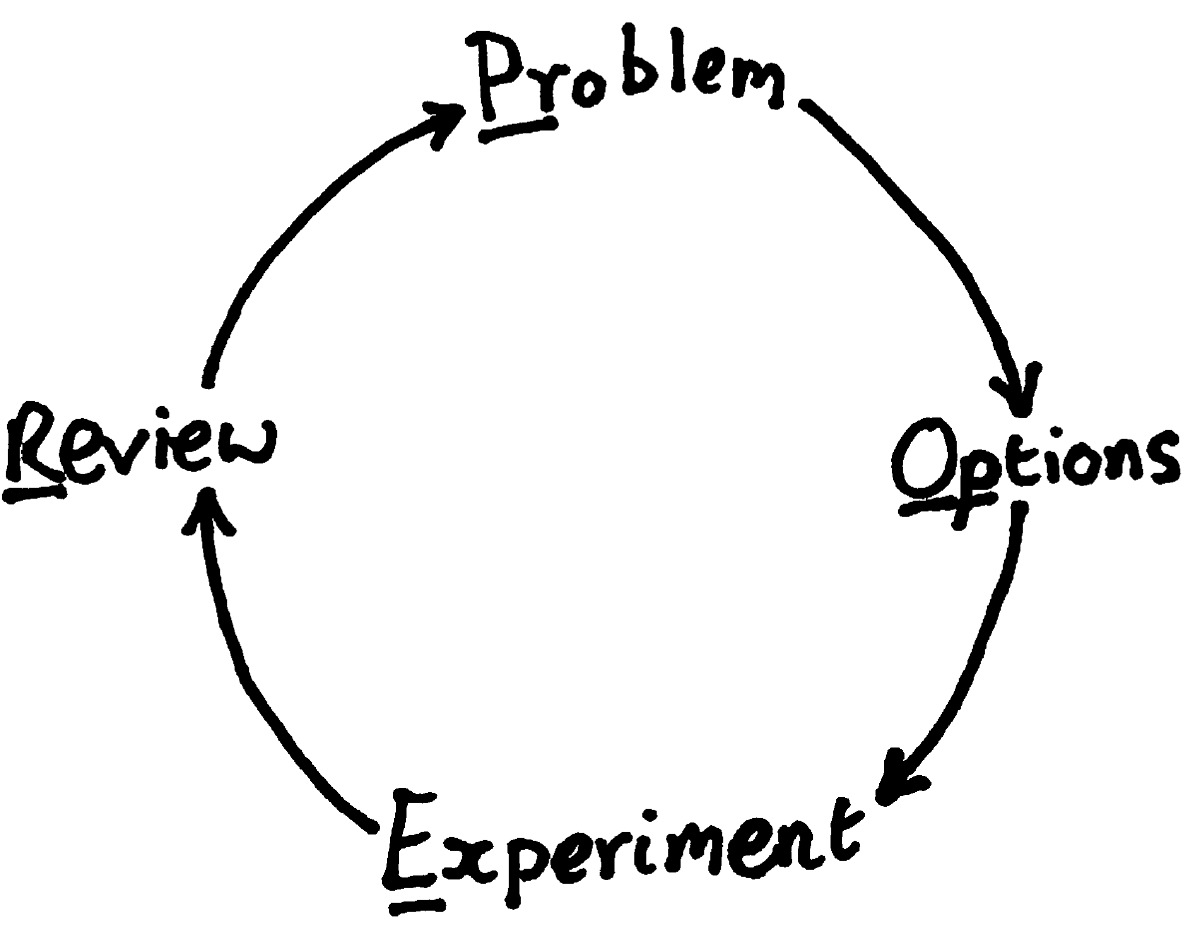
\includegraphics[width=6cm]{PrOpER.png}
        \caption{PrOpER coaching cycle}
    \end{figure}

Não existe lugar certo pra começar. Caso não faça idéia de como começar, faça um brainstorming de idéias para problemas que o projeto tenha. Depois priorize baseado na sua missão como coach -- talvez esse seja o lugar pra começar.

O ciclo \textit{PrOpER}, que significa \textit{Problem, Option, Experiment, Review} e está ilustrado na figura acima, pode ser usado pra atacar cada episódio do seu coaching.
Encontre um \textbf{problema} e veja como a equipe trabalha, veja o que precisa ser melhorado. Considere \textbf{opções}, liste pelo menos três opções pro problema. \textbf{Experimente}, pegue uma das opções e tente. \textbf{Revise}, faça uma revisão do resultado. Você melhorou as coisas? Mesmo que não tenha melhorado, você aprendeu algo?


\section{Mantendo o Passo}
Criar equipes ágeis toma tempo e em alguns dias parece não haver progresso. Se as coisas estiverem indo devagar, não se sinta mal. Tente dar um passo a frente a cada dia.
Caso você tenha problemas com os quais não consiga achar soluções, procure outros coaches fora da sua empresa pra poder trocar experiências. Ao invés de imitar outros coaches, tire proveito do estilo de trabalho deles. Veja como eles lidam com determinadas situações e aprenda, e sempre considere integrar alguma das técnicas deles em sua própria abordagem.



\subsection{Calçando suas Botas de Coach}
Para se sentir confortável dando conselhos como um agile coach leva tempo. Se você desempenhava outro papel na empresa e agora é o coach, vai demorar um pouco até que você consiga deixar sua antiga identidade pra trás.
Se você está fortemente envolvido com tarefas do projeto, será difícil encontrar tempo pra guiar a equipe. Quando alguém faz coach ``pelas laterais'', começando como um player-coach\footnote{Se integra diretamente a equipe, trabalhando junto de cara}, é possível ver o todo de outra perspectiva, podendo focar completamente em melhorar o processo e o trabalho da equipe.

Como saber se você está indo bem como um agile coach?
\begin{itemize}
  \item Olhando pra trás, a equipe está mais agile agora do que um mês atrás?
  \item Você teve boas influências na equipe?
\end{itemize}



\subsection{Indo Adiante}
O que acontece com um pepino se ele ficar num recipiente com água salgada? Ele se torna um picles -- querendo ou não. Em \textit{The Secrets of Consulting}, Jerry Weinberg alerta para o fato de ``tornar-se'' um picles -- se ficamos com a mesma equipe (ou até mesmo empresa) por mais de alguns meses, podemos perder nossa perspectiva. Você pára de notar problemas que eram claros. Você começa a absorver o mesmo comportamento que o resto da empresa e se encontra dizendo, ``Isso é como as coisas são feitas aqui.'.

Se você está ciente de que está ``virando um picles'', tente explicar pra alguém de fora como é o processo da equipe e os desafios que você tem encontrado.

Quando tudo estiver indo bem na equipe, provavelmente seu trabalho como coach está finalizado. A equipe já pode se auto-organizar, e ela precisa parar de depender de você pra dar respostas. É hora de ir adiante!


\section{Impedimentos}
Aqui estão alguns impedimentos que você pode encontrar.

\subsection{Não há tempo pra fazer Coach}
Se você está sobrecarregado com as tarefas da empresa e as pessoas confiam a você determinadas tarefas específicas, você não terá como fazer coach. Não desista do papel de coach. Ao invés disso, trace um plano pra que você não seja mais a pessoa na qual tarefas específicas são confiadas.

\subsection{Falta de Experiência}
Quando você se deparar com uma situação que está fora dos seus conhecimentos, fale abertamente com a equipe ao invés de blefar.

Um coach não precisa ter todas as respostas; as vezes é melhor que não tenha. Ajude a equipe a passar por problemas ajudando na discussão e pesquisando o que outras equipes ágeis estão fazendo dentro e fora da sua empresa.

\subsection{Relutantes a Agile}
Há horas em que nos deparamos com sérios impedimentos pra implantar agile numa equipe. Recomenda-se que você resolva alguns destes impedimentos antes de tentar ser coach, pra evitar certas frustações com os envolvidos no processo.

Às vezes os problemas são técnicas, outrora gerenciais. Tentar implantar ágil numa equipe muito crua pode ser problemático -- é necessário o conhecimento básico de práticas de desenvovimento de software antes de tentar implantar práticas ágeis.

\section{Checklist}
\begin{itemize}
\item Pratique explicar Agile pra ouras pessoas, pode ser qualquer um que queira ouvir.
\item Faça um pequeno estudo pra encontrar a melhor maneira pra ser apresentado à equipe.
\item Encontre maneiras de mostras que você aplica princípios ágeis com você mesmo -- seja o exemplo.
\item Aplique o ciclo PrOpER em suas intervenções.
\item Pause para refletir e aprender com seus erros e faça com que a equipe faça o mesmo.
\item Procure por oportunidades para aprender com outros agile coaches, dentro ou fora da sua empresa
\item Se você trabalhar numa empresa por muito tempo pode acabar se tornando um picles. Quando a equipe estiver pronta, é hora de ir.
\end{itemize}



\chapter{Trabalhando com Pessoas}
Para ajudar equipes ágeis a melhorarem você precisará ouvir cada membro, um por um, para que você possa ver como as melhorias podem ser feitas. Dê feedback pra equipe ver onde podem melhorar.
Esse capítulo abordará habilidades que ajudam a trabalhar com pessoas numa equipe. Você aprenderá como ouvir as pessoas, como lidar com conflitos e criar acordos.


\section{Ouvindo}
Um coach ouve profundamente. Problemas, angústias, idéias que precisam ser refinadas. Tente sempre mostrar pra equipe que você está aberto a ouvir o que eles têm a dizer.

Crie espaço pra que as pessoas possam chegar em você e se abrirem, mostre interesse e sempre mostre que você está ouvindo atentamente o que eles estão dizendo. Quando você ouve com respeito, a pessoa que está falando sabe que você se importa com o que ela diz. Prove que você realmente prestou atenção no que a pessoa falou.

Ouvir atentamente é uma habilidade que você pode aprender. Comece dando total atenção pra quem está falando. Pare tudo que está fazendo e vire-se pra pessoa. Caso a pessoa pareça hesitar em falar abertamente, proponha ir pra algum lugar mais calmo, onde ela se sinta mais à vontade.

Antes de dar qualquer conselho, termine de ouvir. Um grande desafio quando estamos ouvindo alguém é resistir à tentação de começar a aconselhar cedo demais. Foque na pessoa que está falando e tente entender os sentimentos por trás das palavras, sem julgamentos.

\subsection{Lendo nas Entrelinhas}
As pessoas falam muito mais devagar comparado a velocidade que conseguem pensar, por isso é tão difícil dar total atenção quando alguém está falando. Não perca tempo pensando em respostas quando alguém estiver falando. Preste atenção na maneira como a pessoa está falando, na expressão corporal, como se expressam, no tom de voz, pois assim saberá se a pessoa está com raiva, angustiada, feliz ou desconfortável com alguma coisa, e imagine como ela se sente.

\subsection{Mantendo a Confiança}
No fim da conversa, recapitule os pontos-chaves que você ouviu e cheque-os com a pessoa que vos fala. Você entende suas necessidades?

Não traia a confiança dessa pessoa. Pergunte se ela prefere que o que vocês discutiram fique entre vocês ou seja exposto pra equipe analisar.

\subsection{``Background Listening''}
Nem sempre você conversará com as pessoas individualmente, você também terá muitas conversas com a equipe inteira. A maioria das regras citadas acima se aplicam pra conversas em grupos.

Se em algum momento você perceber que há alguns pontos citados nas reuniões que são mal-entendidos você pode escolher em fazer uma pausa na reunião e esclarecer pra todos, ou aguardar até o final pra falar. É interessante sempre ter em mãos papel e caneta pra anotar observações durante a reunião.

\subsection{Dando Feedback}
Quando você observa que algum comportamento não está funcionando pra equipe ou pra algum membro em especial, você naturalmente terá vontade de ajudá-los a ter melhorias. Você precisa compartilhar suas observações, pra que de alguma forma você possa influenciar as pessoas pra que mudem suas atitudes e comportamentos.

Seu primeiro passo pra dar feedback é separar suas informações básicas (o que você viu ou ouviu) de suas avaliações e sentimentos sobre a situação. Fale sobre os acontecimentos da sua perspectiva e dê exemplos específicos do que você viu e ouviu ao invés de interpretações. O quanto mais cedo você disser, melhor, pois é mais fácil pra pessoa falar do que fez e o motivo o quanto mais cedo.

Depois disso é a vez das outras pessoas. Ouça suas versões dos acontecimentos. Talvez exista um bom motivo que explique suas ações e você não sabe.

Caso você veja que ainda é posível fazer mais melhorias, dê sugestões de como eles devem lidar com tais situações no futuro. Peça idéias, também, assim você pode mostrar os prós e contras de cada opção.


\section{Resolvendo Conflitos}
Como coach você pode se ver em situações em que a equipe está presa por confrontos internos. Se você perceber que há conflitos internos na equipe, tire um tempo pra ouvir cada indivíduo.

Antes de agir como um pacificador, veja se o conflito não pode ser resolvido sem sua ajuda. O motivo disso é que se você intervir em cada conflito que surgir, sempre alguém virá choramingar com você, como se fosse um pai chamado pra resolver conflitos entre crianças.

Sempre que você estiver agindo como um mediador, lembre-se que você não pode tomar lados. Ouça cada lado da discussão e mostre que você entende o que está sendo dito, recomeçando a explicação do problema com suas próprias palavras. Explique os fatores que você vê na situação e talvez seja útil estudar as forças envolvidas.

Lembre-se que diferença de opiniões é algo saudável. Muita ênfase em paz e harmonia pode sinalizar que a equipe está sendo complacente. Sempre que for tomar decisões importantes, lembre-se de certificar que você considerou opiniões diferentes.



\section{Criando Acordos}
Quando você introduz novas práticas, é bom saber se todos concordaram com as idéias. Existem equipes em que nem todos compram a idéia da mudança, alguns membros ainda continuam céticos. Uma técnica que ajuda a diferenças de opiniões é a ``gradients of agreement''.

Ao invés de perguntar esperando por um voto de sim ou não, você cria uma escala, onde os extremos são Endossar e Bloquear.

\begin{figure}[h]
    \centering
    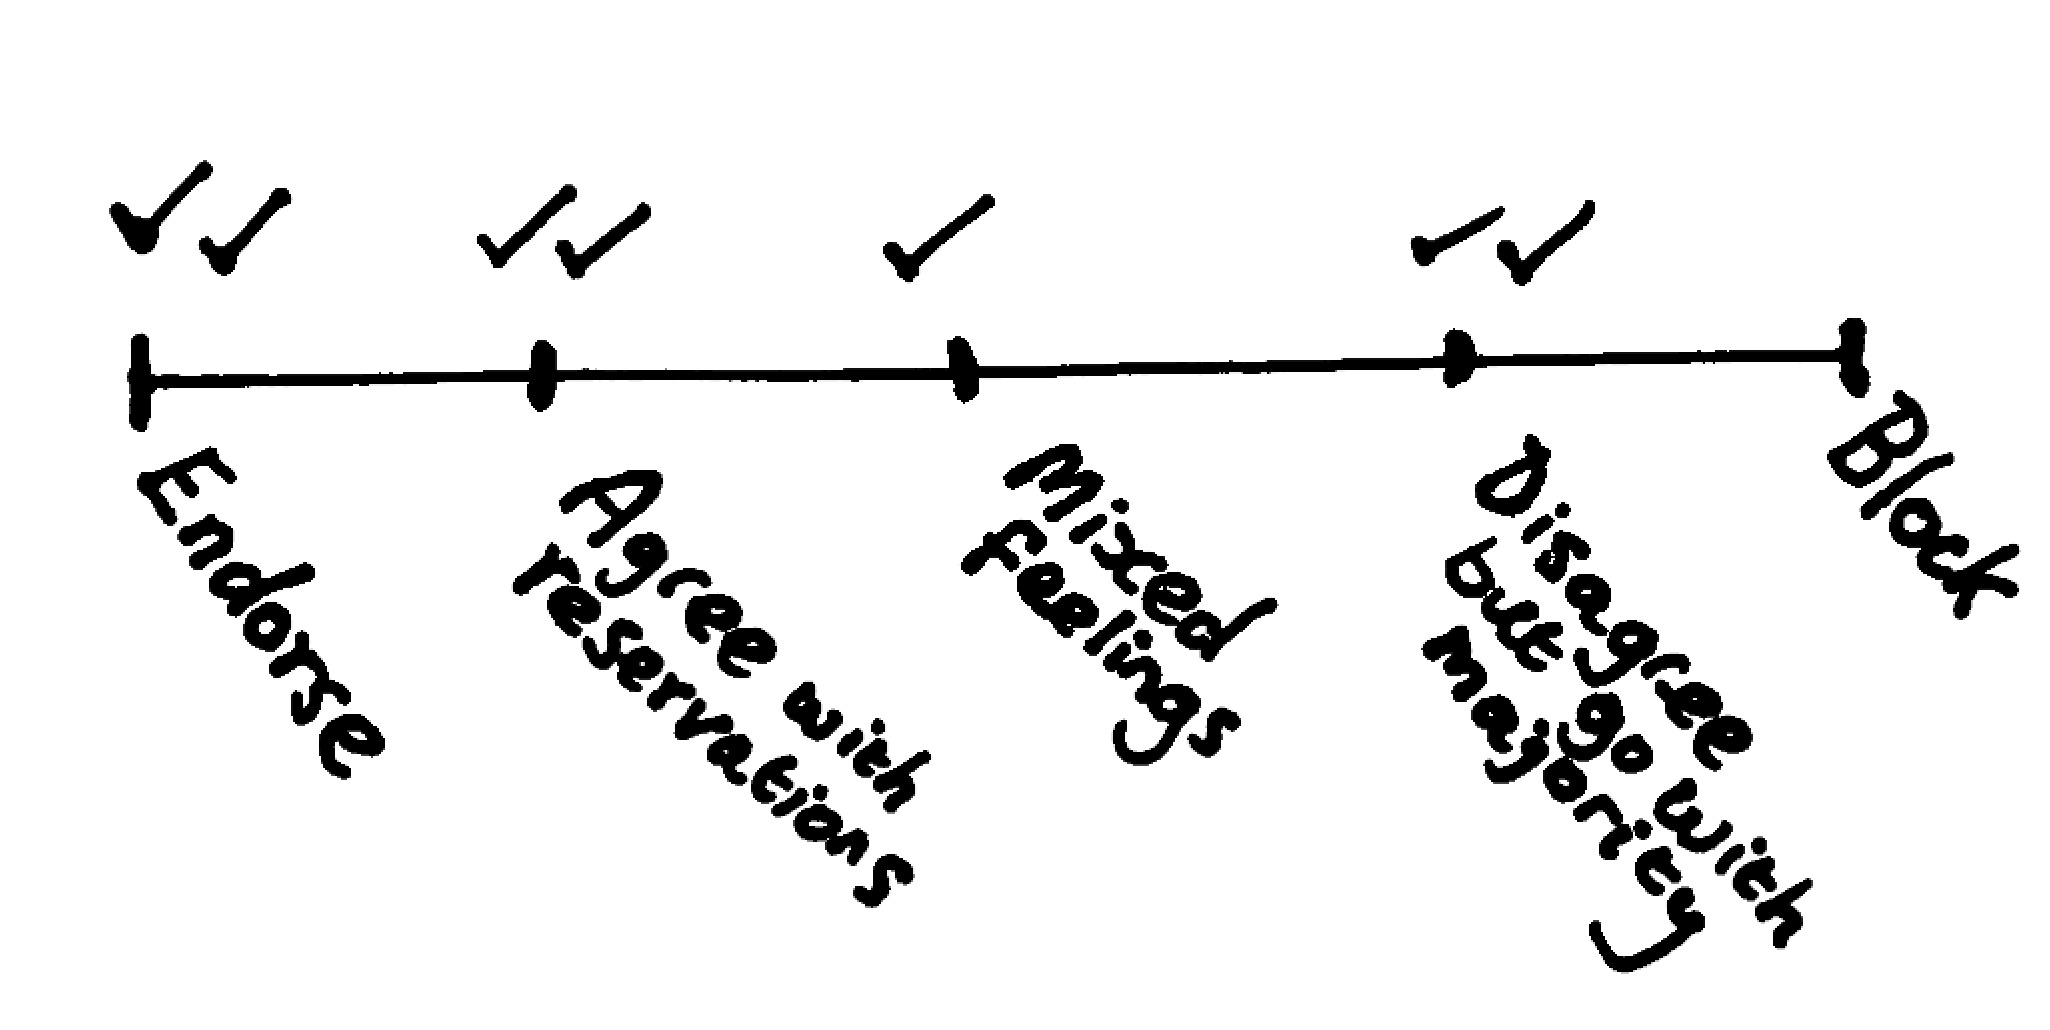
\includegraphics[width=8cm]{gradient_scale}
    \caption{Um exemplo de ``gradient scale''}
\end{figure}

Usar uma escala dessas possibilida descobrir se há alguma falta de consenso. O consenso é importante porque se alguma pessoa não concorda com alguma ação, ela não a implementará entusiasticamente.

A técnica ``gradient scale'' pode ser usada pra estabelecer níveis de concordância entre a equipe. Caso não seja possível usar desenhos da escala, votar em opções de zero a cinco com os dedos da mão também pode ser útil. Independente do método que você escolher, leve-o a sério e pesquise sobre suas preocupações.

\section{Impedimentos}
A seguir estão alguns impedimentos que você pode encontrar.

\subsection{Explosão Emocional numa Reunião}
Caso haja alguma explosão emocional numa reunião, é recomendável que você dê um tempo à pessoa pra que ela recupere sua compostura. Antes de retomar a reunião converse com essa pessoa e entenda seus motivos. Veja se a equipe prefere continuar a reunião ou resolver o problema que causou tal excitação primeiro.

\subsection{Falta de Habilidade das Pessoas}
Algumas pessoas acham que entrando na carreira de desenvolvimento de software não precisarão lidar com pessoas, porque acham isso difícil. Você deve tomar cuidado, pois cada pessoa tem suas preferências em como comunicar-se. Talvez você tenha que ser mais direto com certas pessoas e dar mais espaço a outras.

\subsection{Diferenças Culturais}
Há significados diferentes pra várias coisas em culturas diferentes. Em certas culturas um ``sim'' significa ``Sim, estou escutando'' e não um ``Sim, eu sei como fazer isso.''

Ajude sua equipe a ficar mais antenada com diferenças culturais, tais como tolerância em ambiguidade e individualismo. Uma maneira de fazer isso é estudando o trabalho de Geert Hofstede em dimensões culturais com a equipe\footnote{http://www.geert-hofstede.com/}.

\section{Checklist}
\begin{itemize}
\item Acostume-se a ouvir profundamente pra entender os problemas que aparecem e pra criar confiança. Dê completa atenção às pessoas enquanto conversam e peça esclarecimentos pra ver se você realmente entendeu o que disseram
\item Quando estiver dando feedback, separe o que você viu ou ouviu dos seus sentimentos sobre a situação. Dê exemplos específicos do que você notou, ao invés de comentários. Diga o que você viu ou ouviu, e depois peça explicação dos acontecimentos. Agora junte todos pra ter idéias de como lidar com a mesma situação numa próxima vez.
\item Se um conflito surgir, tenha certeza que todos os lados compartilham seus pontos de vista. Não resolva todos conflitos, senão vão confiar a você o papel de pacificador ao invés de aprenderem com o tempo.
\item Use ``gradients of agreement'' pra descobrir o nível de aceitação de uma mudança. Isso permite que a equipe descubra se existe mais ou menos discordâncias.
\end{itemize}


\chapter{Guiando à Mudança}
Às vezes você estará introduzindo novas práticas ágeis, outras vezes ajudando a equipe a refinar seu processo. De qualquer forma, você precisa guiar a equipe pelas mudanças.

Comece devagar; dê a equipe um tempo pra refletirem sobre as mudanças antes de pressioná-los, e procure oportunidades pra que a equipe aprenda mais sobre agile.

\section{Apresentando a Mudança}
Quando você começar a defender técnicas ágeis pra uma equipe, perceberá que algumas pessoas terão objeções. É natural as pessoas quererem entender melhor os riscos mesmo que tenham um motivo convincente. Conte histórias sobre equipes que obtiveram sucesso com Agile e mostre o que é possível fazer com tais técnicas.

Mostre que você tem confiança na equipe, eles precisam acreditar que você crê neles pra obterem sucesso e isso os encorajará a tomarem o primeiro passo.

Tome cuidado pra não inserir muitas mudanças de uma vez só. Deixe novas idéias aparecerem. É preciso dar tempo à equipe pra conversar e refletir sobre como implementar tais mudanças, nas implicações que poderão surgir, e em como eles encararão isso.


\subsection{Mostre-os Como}
Somente convencer de que a mudança é necessária não é o suficiente pra fazer com que a equipe mude; você precisa mostrá-los como começar. Organize treinamentos pra equipe; demonstre como realizar determinadas tarefas sentando junto, explicando; deixe visível o progresso da equipe.


\subsection{Apresente o Problema}
Como coach, você verá muitas oportunidades pra introduzir melhorias. Porém, antes de compartilhar suas idéias, esteja preparado pra apresentar o problema que está conduzindo a mudança. Deixe claro as implicações que haverão caso a equipe não faça as mudanças necessárias.

Nunca seja grosseiro, pois pode fazer com que o problema pareça difícil demais pra ser superado. Um de seus objetivos é deixar claro as implicações que podem surgir caso a mudança não seja feita. Tome cuidados extras pra não criticar a maneira com qual a equipe trabalha. Seu foco são as melhorias no processo, não em performances individuais.


\subsection{``Build Ownership for Change''}
Uma vez que os problemas foram apresentados, é hora de focar em soluções. Encoraje os membros da equipe a olharem os pontos positivos que melhoraram seu processo ágil. Crie uma propriedade coletiva conversando sobre prós e contras de fazer mudanças.

Deixe que eles saibam as opções que você vê e os convide pra dar novas idéias. Essas conversas se tornam uma parte da vida da equipe uma vez que eles começam a fazer retrospectivas. Uma abordagem em adotar Agile é fazer com que retrospectivas sejam a primeira prática a ser realizada. Retrospectivas provêem a equipe uma série de pontos a serem discutidos e mudanças a serem acrescentadas em poucas semanas.


\subsection{Faça da Mudança um Experimento}
Quando encontrar alguma resistência, proponha tentar algo diferente como um experimento. Encarar uma mudança como um experimento faz com que a equipe foque no benefício, uma vez que a equipe precisa avaliar se o experimento obteve sucesso.

Depois que a equipe decide fazer uma mudança como um experimento, os membros acostumam-se com a nova maneira de trabalhar. Depois disso, voltar pra maneira antiga de trabalho é uma mudança que a equipe hesitará em fazer. Comece com mudanças pequenas, pra que a equipe se prepare para as maiores.

\section{Faça Perguntas}
Outra maneira de liderar uma equipe é fazendo perguntas. Quando você faz uma pergunta a alguém, você demonstra respeito e interesse em sua opinião. Eles precisam forçar o cérebro a pensar numa resposta, e quando fazem isso, caem na sua busca pela melhoria na forma em que a equipe trabalha. Uma pergunta provocativa pode até mesmo fazer com que deêm corda à sua conversa e tomem alguma ação.

Muitas vezes as pessoas se prendem a crenças que acreditam ser verdadeiras. Você pode usar perguntas pra desafiar suas crenças sobre como a empresa trabalha e sobre o que eles podem ou não fazer.

Não faça perguntas que possam ser respondidas com ``sim'' ou ``não''. Faça perguntas que dêem margem à conversa, perguntas como ``Como fazer isso?'', ``O que aconteceria?''; perguntas como estas fazem com que a pessoa reflita e compartilhe seus pensamentos.

Cuidado com com perguntas que tenham ``Por quê?'', pois podem parecer críticas a idéias ou até mesmo acusações. Por quês tendem a tratar de problemas, e não de soluções.

\subsection{O que Perguntar ou Pedir}
Existem vários tipos de perguntas e pedidos, a seguir há alguns interessantes.

\subsubsection{Peça Ajuda}
Peça ajuda a alguém de uma forma mais pessoal, evite fazer isso em reuniões. Mostre algum problema com o qual você está lidando e peça ajuda. A pessoa pode oferecer idéias, suporte ou até mesmo algo mais prático. A maioria das pessoas ama ajudar e se sentirão lisonjeados em te ajudar.

\subsubsection{Perguntas Intrigantes}
Você pode facilitar o raciocínio de alguém fazendo perguntas intrigantes. Tais perguntas forçam a pessoa a desfocar dos detalhes do problema e olhar para o problema de uma perspectiva diferente.

\subsubsection{Perguntas que Fazem Refletir}
Incentive a equipe a notar mais em como eles trabalham, fazendo, mais a frente, perguntas sobre o que eles notaram. Compartilhe suas observações pra ajudá-los a entender o seu interesse. Pegue experiências do dia-a-dia, as observações dos membros da equipe e procurem, juntos, por melhorias baseado no que foi bom ou ruim.

\subsubsection{Cinco Por Quês}
A técnica dos Cinco Por Quês \textit{(Five Whys)} foi inventada por Taiichi Ohno, e pode ser usada pra achar a raiz de algum problema. A técnica consiste em pegar um problema aparente, depois perguntar o que causou tal problema, o que causou o último, e o último, e o último e o último. Quando você tiver perguntado ``Por quê'' cinco vezes, achará o problema real, que será um problema sistemático. É importante explicar pra equipe a técnica, pra não parecer que os por quês estão sendo repetidos por descontentamento com a resposta.


\subsection{Quando Não Fazer Perguntas}
Evite fazer perguntas quando você quer dar orientações para alguém da equipe. Se você fizer alguma pergunta, terá que aceitar a resposta, e se você discordar, será mais difícil dar o conselho que você queria.

Se você só faz perguntas, deveria compartilhar mais o que você sabe, senão as pessoas não se abrirão pra você. Tenha em mente que se você não se importa com a resposta, quando você fizer alguma pergunta, poderá parecer que está tentando apontar falhas em alguém.

Não faça perguntas pra determinada pessoa se existir pouca confiança entre vocês. Certamente essa pessoa reagirá defensivamente e a resposta não será verdadeira. Ao invés de perguntas, nesses casos é melhor uma conversa aberta e direta.


\section{Apoie o Aprendizado}
Sua equipe precisa aprender sobre Agile antes de adotar práticas ágeis. Encoraje-os pra que se dediquem a estudar um pouco sobre agile, seja no tempo de trabalho ou em casa. Faça com que eles tomem a iniciativa pra aprenderem por si próprios ao invés de dependerem de você como fonte de conhecimento sobre Agile.


\subsection{Crie Oportunidades de Aprendizado}
As idéias ágeis ainda em expansão, estão evoluindo, assim, você precisa estar sempre atualizado sobre o que está acontecendo ao redor do movimento ágil. Existem várias maneiras de aprender sobre Agile, e uma de suas funções é tornar isso fácil.

Uma maneira eficiente de apresentar idéias sobre Agile é organizando apresentações com membros da própria empresa, pra falarem sobre suas experiências com Agile. É uma maneira de criar oportunidades pra que amigos de trabalho possam mostrar o que aprenderam sobre Agile, além de dar oportunidades de falarem em público.

Você pode também convidar pessoas de fora, experts da área ou conhecidos de grupos locais sobre agile, pra compartilharem com você e sua equipe experiências de como usaram ou usam Agile em algum projeto ou empresa.


\subsection{Indo Para Fora da Empresa Para Aprender}
Conferências são uma ótima maneira de expôr a equipe a novas idéias, porque lá haverá pessoas com mesmos problemas, pessoas que compartilham suas experiências, e sempre é possível encontrar ajuda. Inclusive é uma maneira de abrir os olhos de quem está na empresa por muito tempo.

Sua equipe pode também encontrar ajuda e novas idéias em grupos locais sobre agile. Ao invés de informá-los sobre o próximo encontro que você irá, convide-os pra ir com você.


\subsection{Facilitando Reuniões}
Sempre que uma nova mudança estiver pra ser implantada, mostre a equipe como se faz. Na primeira vez que uma equipe ágil fizer uma reunião, seja uma retrospectiva ou uma reunião de planejamento, ofereça-se pra facilitar a reunião, pra mostrá-los como é feito. Durante a reunião explique como o processo funciona, pra que numa próxima vez eles possam fazer sozinhos. Da próxima vez, planeje junto da pessoa que será o facilitador da reunião, e durante a reunião não interrompa até que a reunião termine -- a não ser que comece a sair do foco.

Após a reunião, exponha suas idéias do processo e pra ser melhor ainda na próxima vez, peça feedback da equipe.

Pra tornar a reunião eficaz, você precisa:
\begin{itemize}
\item escolher um horário que seja adequado a todos da equipe
\item arrumar um lugar adequado pra fazer a reunião
\item manter sempre o foco da reunião
\item manter a reunião fluindo, tornando-a fácil para as pessoas
\item encoraje todos a participar com idéias, opiniões, dúvidas ou respostas
\item resuma os pontos principais pra ter certeza que tudo foi bem compreendido
\item termine a reunião tendo certeza que o que foi gerado na reunião tenha sido devidamente gravado
\end{itemize}


\section{Impedimentos}

\subsection{Algumas Pessoas Nunca Mudam}
Algumas pessoas gostam de ser as primeiras a acolher amudança, outras preferem ser as últimas. Não se prenda a essas pessoas, elas gostam de ser as últimas. Quando Agile for o padrão, tenha certeza que elas adotarão.


\subsection{Dando de Cara com as Políticas da Empresa}
Quando a mudança começa a ser feita, você irá dar de cara com políticas internas da empresa. Algumas pessoas -- gerentes de projeto, arquitetos -- podem achar que seus emprego correm perigo. Procure mal-entendidos e tente resolvê-los.

Um líder técnico pode ser um impecílio na mudança da equipe pra Agile, e nada ajudará se você for muito crítico sobre essa pessoa. Invista algum tempo entendendo a perspectiva da pessoa, só assim você irá conseguir argumentos pra convencê-lo com seus planos sobre da mudança.


\subsection{Planos de Trabalhos Conflitantes}
Às vezes é difícil manter o foco quando outras pessoas estão esperando que você resolva seus problemas. Por exemplo, alguém veio reclamar sobre não poder colar nada na parede. Você pode concordar que é um problema, mas talvez não seja a hora certa pra resolver isto.

Tente ser neutro em público e explique em particular sobre o que você tem feito pra tentar resolver os problemas, evitando ficar com reputação de pessoa negativa. Explique os problemas que você tem no momento e peça que alguém te ajude. Depois você deve avaliar se vale a pena se esforçar pra resolver os problemas, ou chegar a conclusão de que não é uma boa hora.


\section{Checklist}
\begin{itemize}
\item Converse sobre agile, demonstre, ofereça-se pra ajudar as pessoas; encoraje e inspire, mostrando que Agile pode funcionar para a equipe
\item Apresente o problema pra equipe; ajude-os a enxergar o motivo da mudança; converse individualmente com os membros da equipe
\item Quando se deparar com alguma resistência, tente entender de onde ela vem. Veja se foi por causa da forma com a qual alguma idéia foi apresentada; veja se existem bons motivos pras pessoas se preocuparem com a idéia proposta; e observe se você tem prestado atenção nas observações da equipe
\item Faça perguntas pra forçar a equipe a melhorar seu processo ágil. Peça ajuda, faça perguntas intrigantes, perguntas que façam as pessoas refletirem, use a técnica dos ``Cinco Porquês''
\item Apoie novas maneiras de aprender sobre agile: livros, blogs, podcasts. Organize apresentações, grupos de estudo. Deixe-os informados sobre eventos sobre Agile e leve-os pra grupos locais sobre Agile
\item Faça com que novas reuniões sejam fáceis, sendo o facilitador na primeira vez. Exponha suas idéias sobre o processo da reunião. Ajude a equipe a preparar a próxima reunião, e depois dê a eles feedback
\end{itemize}




\chapter{Montando Uma Equipe Ágil}
Equipes ágeis não aparecem do nada, leva tempo pra equipe ser formada. Quando uma equipe não se une, as pessoas ficam frustadas e o software que eles produzem reflete isso.

Você pode ajudar uma equipe a ser mais unida fazendo com que os membros se conheçam melhor e melhorando o ambiente de trabalho. Procure maneiras pra ajudar a equipe inteira saber aonde o projeto está indo.

\section{Ajudando uma Equipe a se Unir}

\subsection{O Lado Social}
Fazer com que uma equipe seja unida e que os membros confiem uns nos outros, leva tempo. Trabalhando junto a equipe começa a entender as perspectivas e problemas uns dos outros. Encontros, em especial o Daily Standup (ou Standup Meeting) e retrospectivas, são uma oportunidade pra equipe se conhecer melhor.

Você deve criar oportunidades pra equipe se conhecer melhor, seja trocando histórias pessoais ou saindo junto.

\subsection{Crie Confiança}
Trabalho em equipe cria confiança. Você pode guiar a equipe a criar confiança uns nos outros mostrando que é seguro se abrir. Seja transparente sobre motivos, exponha informações sobre experiência, sentimentos e opiniões -- isso faz com que as pessoas também se abram. Admita quando você errar. Peça ajuda regularmente.

Caso exista no ambiente de trabalho algum costume de punir ou criticar alguém quando errarem, isso fará com que as pessoas não se sintam seguras. Os membros da equipe precisam se sentir confortáveis pra dizer quando precisam de ajuda, e quando isso acontecer eles se sentirão felizes em compartilhar conselhos e ajudar os amigos de equipe.

Se as pessoas se sentirem inseguras -- se estiverem com medo de serem demitidas, por exemplo -- você não conseguirá fazer nenhum agile coaching. Nesse caso, você precisa dar suporte à equipe da maneira que puder até que a situação se resolva.


\subsection{Preenchendo a Lacuna}
Criar confiança entre pessoas com cargos diferentes é mais difícil do que entre pessoas com o mesmo cargo. Você pode sugerir que as pessoas troquem de papel por um perído curto de tempo, pra verem como é o trabalho da outra pessoa. Um desenvolvedor poderia ficar por uma semana como testador, por exemplo (caso possua os conhecimentos necessários), ou parear com um testador contribuindo com o máximo possível.

Às vezes por não entenderem direito o trabalho do outro, as pessoas assumem que o seu próprio trabalho é mais difícil. Sem respeito mútuo uma equipe não será bem sucedida. Você pode demonstrar respeito pelas pessoas pedindo opiniões ou ajuda e levando seus interesses e idéias a sério. Outros notarão e imitarão você.

Se uma pessoa parece estar infeliz com outra, convide-a para um café e discuta isso. Quais suposições que fizeram isso acontecer? Quais explicações possíveis existem pra isso?


\section{Criando um Bom Ambiente Para a Equipe}
Uma equipe precisa de um ambiente de trabalho compartilhado pra fazer com que a informação flua. O ideal é que toda a equipe trabalhe na mesma sala. Uma área pequena perto da equipe, onde eles possam tomar um café ou conversar, melhora o entrosamento entre a equipe. Uma sala de reuniões próxima é útil por questões de privacidade e pra discussões que não atrapalhem a equipe. Esse passo é crucial pra fazer uma equipe ágil dar certo. Todos devem trabalhar na mesma sala, sempre.

Se algumas pessoas não concordarem com esta idéia, encoraje-os a personalizar seu lugar de trabalho, seja com livros, plantas ou fotos, pra que elas se sintam à vontande pra trabalhar.

Vale lembrar que você não deve se preocupar só com o espaço físico. O ambiente virtual também deve ser levado em conta. Encoraje a equipe a ter uma wiki ou repositórios de documentos compartilhados. Eles também precisam estar a par do setup do ambiente de desenvolvimento e de testes.


\section{Equilibrando Papéis}
A relação entre clientes e desenvolvedores é crucial, porque eles precisam trabalhar juntos pra criar o melhor produto. Todos precisam se sentir parte da mesma equipe, trabalhando com o mesmo objetivo final. Deixe claro as responsabilidades de cada um pra equipe toda.

O cliente (\textit{customer}, ou \textit{product owner} no Scrum) é a pessoa responsável por priorizar o que o software deve fazer. A equipe de desenvolvimento é responsável por decidir como criar o software e dizer ao cliente o tempo que levará. O cliente pode definir datas pra que o software seja entregue, mas não pode tornar o escopo fixo -- o escopo é definido em equipe.

Normalmente o cliente é um gerente de produtos (\textit{product manager}) que trabalha com vários usuários e \textit{stakeholders}\footnote{stakeholders são os clientes reais, as pessoas que pagam pelo software} pra decidir o que o software deve fazer. Em desenvolvimentos grandes, o papel de cliente pode ser demais pra uma pessoa só, assim é formada uma equipe que representará o cliente. Essa equipe deve ter a expertise necessária pra lidar com user stories e priorizá-las, e pode ser formada por analistas de negócio, representantes do usuário ou designers de interação, dependerá do projeto.

Às vezes a melhor solução é um ``cliente-perto'' (\textit{near-customer}), que ajuda a trabalhar nos detalhesdos requisitos com a equipe, e um ``cliente-longe'' (\textit{far-customer}) que toma decisões sobre as prioridades do negócio. O cliente-perto pode ser um analista de negócios que fica perto da equipe, enquanto o cliente-longe pode ser um gerente de produtos que fica perto das operações do negócio e das equipes de marketing.

Se os papéis saírem do equilíbrio, um dos lados terá trabalho em excesso. Se o excesso estiver do lado do cliente, os desenvolvedores não terão tempo suficiente e terão que adivinhar o que o cliente quer. Se não houver desenvolvedores suficiente, ou estiverem trabalhando mais devagar do que o esperado, a parte de negócio se desapontará com os resultados. Como coach, você pode ajudar fazendo com que os efeitos colatereais do desequilíbrio sejam mais visíveis. Assim, a gerência pode pensar em como resolver tais problemas.



\section{Energizando a Equipe}
A seguir estão algumas idéias de como energizar a equipe e ajudá-los a encontrar sua própria motivação.


\subsection{Nem Tão Fácil, Nem Tão Difícil}
Todo mundo precisa ser suficientemente desafiado -- nem entediado, nem ansioso. Essa é a parte do trabalho que as pessoas mais gostam.

Se for muito fácil, os desenvolvedores ficarão entediados e desmotivados. Se houver muitas coisas fáceis a serem feitas, encoraje-os a criar soluções automatizadas.

Às vezes o trabalho parece impossível de ser feito e as pessoas acabam travando no problema. Quando isso acontecer, é necessário dividir o problema em partes mais gerenciáveis, para que a equipe consiga pegar alguma coisa pra começar.

Sustente uma cultura onde não há problemas em experimentar e aprender sobre um problema que precisa ser resolvido. Às vezes a equipe pode achar que perdeu tempo com experimentos, mas é uma maneira rápida de aprender e muito barata de avaliar os custos da decisão errada.


\subsection{Encontre um Objetivo Atrativo}
Saber que a equipe está criando um produto que é útil ajuda a equipe a se empenhar melhor. Se possível, arranje um encontro entre a equipe e usuários finais. As necessidades dos usuários serão mais claras pra equipe e darão idéias de como eles podem ajudar a fazer um produto melhor.

Equipes ágeis planejam e gerenciam seu próprio trabalho. Uma vez que a equipe entender que eles não precisam esperar por permissões, ficarão livres pra começar a andar com as próprias pernas.


\subsection{Tempo pra Inovação}
Quando membros de uma equipe ágil trabalham sem parar num fluxo contínuo de user stories, a equipe pode acabar sendo prejudicada.

Se as pessoas não tiverem tempo pra explorar ou aprender alguma coisa nova, elas podem se sentir desmotivadas. Deixe um tempo no planejamento da iteração pra equipe explorar novas idéias.

Quando os membros da equipe têm tempo pra buscar por inovação, eles ficam mais felizes no trabalho. Isso melhora a energia da equipe e remove atrito de tarefas relacionadas ao projeto. Incentive a inovação dentro da equipe, deixando tempo reservado pra cada um. Use de técnicas como \textit{Gold Cards}\footnote{veja ``Innovation and Sustainability with Gold Cards'' apresentado na XP Universe 2001 Conference} pra que cada membro sinta-se a vontade pra ficar um dia por conta de aprender alguma coisa nova e no fim da iteração compartilhar o que aprendeu.


\subsection{Celebre o Sucesso}
Encontre maneiras de celebrar o sucesso a cada release. Saia com a equipe pra almoçar, beber ou até mesmo comer uma pizza. A comemoração aumenta os laços entre a equipe.

Ajude a equipe a mostrar para pessoas de fora seu sucessso. Faça apresentações de demonstração, mande convites pra pessoas de fora. Uma palavra de obrigado dos clientes é sempre bem vinda e aumenta o moral da equipe.


\subsection{Não Desmotive}
As pessoas começam motivadas. Se nada as desmotivar, elas tendem a continuar motivadas! O motivo de as pessoas continuarem motivadas é o que elas fazem. E o que faz as pessoas ficarem desmotivadas é a situação com que elas trabalham -- incluindo estresse e cultura da empresa.

Computadores rápidos e um café decente não seriam notados se sempre estivessem lá. Porém, a falta deles poderia desmotivar os membros da equipe. Como coach você talvez não possa influenciar diretamente nisso, mas vale a pena conversar com a equipe pra ver o que os incomoda. Você pode encontrar coisas fáceis de resolver, como melhorar o ambiente de trabalho.


\subsection{Cuidado Com Os Incentivos}
Tenha cuida ao usar ``incentivos'' pra motivar pessoas. Esquemas de incentivos pessoais podem atrapalhar o trabalho em equipe, pois ajudar os colegas de trabalho não faria sentido se todos estivessem concorrendo a um bônus.

Caso um bônus seja oferecido pra equipe quando uma tarefa for terminada, nada mais nada menos do que o que for preciso fazer pra ganhar o bonus será feito. Se a gerência tem um esquema de bônus, converse com eles pra que esse bônus não tenha como foco indivíduos isolados, mas a equipe como um todo. A equipe produzirá mais e fará um produto melhor quando estiverem motivados.



\section{Impedimentos}

\subsection{Equipes Não São Especialista-Generalistas (\textit{Cross-Functional})}
Algumas empresas organizam equipes por disciplinas, como testadores, desenvolvedores, analistas, designers e etc. Isso é um grande bloqueador na transição pra Agile, porque um dos princípios ágeis é equipes especialista-generalistas (\textit{crosss-functional}), com diferentes disciplinas, que desenvolvem junto o melhor software possível.


\subsection{Não Há Cliente Presente}
Às vezes a equipe de desenvolvimento está num lugar e o cliente em outro. Se não manejado bem, o cliente remoto pode ser um grande problema na comunicação da equipe.

Criar uma boa comunicação com o cliente remoto nesse caso, é vital. Encoraje o cliente a se encontrar pessoalmente com a equipe, pra que todos possam se conhecer. Isso pode ser feito na primeira reunião de planejamento. Depois disso você pode encorajar conversas por telefone ou chat na internet, de preferência com webcam -- pra que todos possam se ver e criar um clima mais amigável.


\subsection{A Equipe É Grande Demais}
Se você está trabalhando com uma equipe com mais de dez pessoas, está propício a ter problemas com comunicação e responsabilidades dentro da equipe. Qualquer reunião se torna mais longa, e os membros se sentem menos motivados por parecem pouco dentro da equipe. Trabalhe com a equipe pra dividi-la em subequipes -- idealmente equipes centradas nas funcionalidades do cliente (\textit{feature teams})\footnote{veja Scaling Lean \& Agile Development, 2009}.


\subsection{A Equipe É Um Conjunto de Recursos}
Agile não funciona bem quando um conjunto de pessoas trabalhando em vários projetos tenta aplicar Agile como se fossem uma equipe só. Agile assume um projeto por vez. Quando a equipe trabalha em vários projeots, não há grandes objetivos que são atrativos. Você nota que prioridades em diferentes projetos mudam, e isso causa interrupções que deveriam ser trabalhadas dentro da equipe. Recomenda-se não aplicar Agile nessa situação.



\subsection{Os Membros da Equipe Isolam Alguém da Equipe}
Você pode notar que a equipe está evitando trabalhar com uma determinada pessoa. Será que é um problema de falta de confiança? Ou seria um problema prático? Talvez porque a pesssoa não tomou banho de manhã?

Tente conversar com a equipe (quando a pessoa isolada não estiver por perto) pra ver qual é o motivo do isolamento. Depois converse com a pessoa em questão, veja se ela está sabendo da situação. Envolva o departamento de Recursos Humanos caso você perceba que a pessoa está distraída por questões de doença, estresse ou depressão.

\subsection{A Equipe se Torna Complacente}
Equipes ficam cheias de si mesmas quando não há exposição para outras equipes e objetivos dos négocios. Se você notar que a equipe está ficando muito complacente, vale a pena tentar aumentar a visibilidade do trabalho da equipe para os stakeholders e aumentar o feedback para a equipe sobre os valores gerados por seu trabalho pros negócios.



\section{Checklist}

\begin{itemize}
\item Crie oportunidades pros membros da equipe se conhecerem melhor, o que a ajuda a equipe ser mais unida. Regularmente gaste um tempo informal juntos, como almoços ou drinks.

\item Crie um ambiente de trabalho compartilhado pra ajudar a equipe trabalhar bem junta. Tente fazer com que toda a equipe fique na mesma sala.

\item Deixe claro as responsabilidades de cada papel. Consiga com o cliente o suporte necessário pra trabalhar dentro da equipe.

\item Garanta que a equipe tem um objetivo alcançável, mas desafiador. Tenha certeza que o trabalho não é nem muito fácil, nem muito difícil.

\item Consiga comida e bebida pra celebrar cada release. Peça aos clientes e gerentes pra agradecerem a equipe.

\end{itemize}



\part{Planejando Como Uma Equipe}

\chapter{Daily Standup (Standup Meeting)}
Daily Standup é a reunião diária que a equipe deve fazer. Cada membro deve responder a três perguntas:
\begin{itemize}
\item O que você fez ontem?
\item O que você fará hoje?
\item O que está te atrapalhando?
\end{itemize}

Nessas reuniões diárias todos devem estar de pé -- pra evitar que se prolongue muito --, e não deve demorar nem meia hora (em média são menos de 15 minutos). Como coach, você deve procurar adaptar as perguntas básicas para as necessidades de sua equipe, pois nem sempre as perguntas citadas acima são suficientes.

Alguns sinais demonstram se a equipe está trabalhando bem nas reuniões diárias. Veja se todos estão interessados durante a reunião, se não está entrando em muitos detalhes que só estão fazendo a reunião ser mais longa, e repare se a equipe faz reuniões diárias mesmo quando você não está por perto. Quando elas forem rápidas, enérgicas, e gerenciadas sozinhas, a equipe estará no caminho certo.

Achar o equilíbrio nas reuniões diárias é uma arte. A seguir serão apresentadas algumas maneiras de melhorar tais reuniões.


\section{Ficando de Pé}
Talvez a equipe ache desconfortável ficar em pé nas reuniões. Mostre a eles o motivo de ficarem de pé. Todos devem entender que a reunião é em pé pra que não se prolongue por muito tempo.

Caso eles sejam relutantes a esta idéia, faça um experimento. Faça com que a equipe tenha pelo menos daily standups por duas semanas e depois avaliem juntos os resultados. Caso a equipe concorde com a idéia das reuniões diárias, mas acabe se sentando em algum momento, monitore o tempo que a reunião durou quando estavam sentados e quando estavam de pé.

Prefira fazer daily standups na sala da equipe, onde tenha um quadro branco e o quadro de tarefas seja visível. Evite fazer tais reuniões em outras salas, pois assim, evita-se o tempo de ir e vir.

\section{Para a Equipe, Pela Equipe}
É essencial que a equipe consiga transmitir a mensagem através de daily standups. A equipe precisa entender que as daily standups são feitas pra sincronizá-los com seu próprio trabalho.

Mantenha a conversa focada no que foi planejado; não deixe que a conversa desvie pra algo que não tem a ver com o plano -- como o que alguém fez no fim de semana ou nas férias. Seja educado, e caso necessário lembre a equipe dos objetivos das daily standups.


\subsection{Estabelecendo um Foco}
Observe -- se você perceber que você tem feito as perguntas nas reuniões diárias, verá que as respostas acabam sendo direcionadas a você, e não à equipe inteira, como se o benefício da reunião fosse seu, e não deles. Quando isso acontecer, tente não olhar fixamente pra uma pessoa só, olhe pra todos da equipe.

Se em algum momento você perceber que as pessoas têm tratado a reunião como um relatório pra você, pare e diga: ``Por favor, direcionem as respostas pro grupo. A reunião é pra todos saberem o que vocês precisam fazer hoje, não eu.'' Outra alternativa é não comparecer às daily standups, deixando a equipe fazê-las sozinha.

Evite agradecer ou dizer ``ótimo'', ou ``bom trabalho'' depois que alguém terminar de falar. Se você fizer isso, reenforçará a idéia de que o objetivo da reunião diária é sincronizar as atividades da equipe, e não te agradar.


\subsection{A Equipe Controla o Andamento}
Encoraje a equipe a tomar conta das suas daily standups. Para tornar isso explícito, apresente um \textit{token}\footnote{algum objeto que deixe claro quem tem o direito de falar} que é passado de pessoa pra pessoa. O token pode ser qualquer objeto, como uma bola, um boneco, um marcador de texto, etc que a pessoa com o direito de falar segura. A pessoa com o token tem o direito de escolher quem será o próximo a falar.


\subsection{Quem Faz Parte}
A equipe inteira deve ir à daily standup: desenvolvedores, testadores, designers, cliente, coach, e assim por diante. Em alguns lugares, os stakeholders não podem falar nada nas daily standups. Desencoraje a idéia de que os clientes não podem falar. A equipe precisa se relacionar bem e se manter atualizada com os clientes.

O foco das daily standups é trabalhar no plano corrente e é a hora ideal para os clientes passarem informações sobre o que estar por vir. Tais atualizações devem vir no fim da reunião.

Evite falar sobre o que não interessa a equipe inteira, mas não se esqueça de conversar com as pessoas interessadas após a daily standup.

\section{Lidando com Problemas}
Quando alguém menciona algum problema que está tendo, é melhor deixar a discussão de como resolver tal problema para o fim da reunião. O motivo é que ninguém terá a idéia do todo antes do fim. Assim, pode ser que antes do fim da reunião seja dito algo que solucione ou ajude na solução do problema. Outro ponto é que nem todos são necessários pra resolver cada problema. Tente separar conversas nas daily standups.

Quando alguém citar algum problema, escreva-o no quadro para que todos possam ver. Ao fim da reunião priorize os item que estiverem no quadro e assim que forem resolvendo, risque-os. Não há necessidade de manter um log de tais problemas, a não ser que esteja havendo muitas interrupções de pessoas de fora.

As daily standups não devem substituir outras reuniões. Caso haja necessidade de uma discussão mais longa com a equipe inteira, marque uma reunião sobre tal assunto, ao invés de conversar no fim da daily standup.


\section{Escolhendo um Horário}
A maioria das equipes prefere que as daily standups sejam no início do dia de trabalho. Porém, em algumas equipes isso não é possível -- há equipes que são distribuídas pelo mundo, com fuso horários diferentes, pessoas que trabalham em diferentes períodos do dia.

Como coach, você não deve escolher o horário da reunião. Deve ser uma decisão da equipe. Isso não fará com que a decisão seja mais fácil, mas deixará com eles a responsabilidade e promoverá a cultura de a equipe resolver seus problemas sozinha.


\section{Quando Fazer Coach}
Se você não está direcionando as conversas na daily standup e as reuniões demoram muito, onde você está agregando valor como coach? A idéia é que o coach seja a consciência da equipe. Você pode, por exemplo, gentilmente relembrar à equipe o que eles planejaram, caso eles estejam fugindo do planejado. Você não pode ser chato e ficar toda hora dizendo "Não equeça isso", "Não esqueça aquilo". Espere que eles fiquem à deriva, depois faça algumas observações do que você vê a equipe fazer é diferente do que havia sido planejado. Veja com a equipe se há algum problema, e caso exista, conversem pra ver como lidar com isso.

Os membros da equipe passam tanto tempo implementando user stories que acabam não vendo o tempo passar. Você pode relembrá-los de quantos dias faltam para a próxima apresentação de demonstração ou release, para que assim vocês possam ver juntos se o que está no quadro reflete o que está sendo feito.

A equipe está trabalhando num ciclo iterativo. Assim, eles não podem se esquecer de pegar um tempo em cada iteração pra escrever novas user stories junto ao cliente para a próxima release planning. A equipe precisa trabalhar no que foi levantado nas restrospectivas até o fim da iteração.

Às vezes a equipe não discute problemas por acharem que não podem ser resolvidos ou por terem se acostumados. Estude a equipe através das formas não verbais, como linguagem corporal.

\begin{itemize}
\item Todo mundo está engajado, motivado e animados?
\item Estão fazendo progresso e trabalhando nas tarefas de maior prioridade?
\item Estão trabalhando juntos e se ajudando?
\item É possível que a equipe se concentre e trabalhe sem interrupções?
\end{itemize}

A não ser que você esteja seriamente preocupado com a perda de foco da equipe, siga essas observações depois da reunião, ou deixe para a próxima retrospectiva.


\section{Impedimentos}

\subsection{Pessoas Chegam Tarde Para a Reunião}
Não repita o que foi dito pra quem chegar atrasado. Além de ser desrespeitoso com os que estavam no horário correto, parecerá que não há problemas em chegar atrasado.

Há equipes que concordam com que as pessoas que chegam atrasadas paguem uma pequena quantia em dinheiro, e depois o dinheiro é usado pra equipe sair pra comer ou beber juntos. Essa abordagem precisa de muito cuidado pra ser usada, pois algumas pessoas podem se sentir à vontade pagando uma pequena taxa e chegando atrasadas.

Se alguma pessoa constantemente chega atrasada, converse com ela sobre isso e tente entender o problema. Porém, independente do problema, algo precisa ser feito pra que tal pessoa esteja presente nas reuniões.


\subsection{Reuniões Demoram Muito}
Se a daily standup leva mais de quinze minutos, procure maneiras de torná-la mais rápida. É recomendável que nesse caso se prendam às perguntas básicas, com cada um respondendo às perguntas e deixando as discussões pro fim.

Relembre que não há necessidade de cada um falar sobre cada detalhe do que foi feito ontem; o que deve ser discutido é apenas o que é importante pra que todos da equipe fiquem atualizados do produto como um todo. Foque no que é relevante para que as tarefas mais relevantes sejam cumpridas hoje e o que precisa ser feito pra que tudo fique no prazo.

Caso a equipe seja grande (com mais de dez pessoas), as daily standups podem acabar fazendo com que alguns membros fiquem entendiados, não ouçam aos outros e a equipe acaba perdendo os benefícios da daily standup. Você pode fazer com que as perguntas sejam feitas sobre cada user story do quadro, ao invés de fazer perguntas individuais.

A melhor alternativa pra equipes grandes é dividí-la em subequipes, que planejam separadamente e tem daily standups mais curtas. Assim, as subequipes coordenam seu trabalho através de uma nova reunião chamada \textit{scum of scrums}.



\subsection{A Daily Standup É Roubada}
A reunião diária pode ser sequestrada por alguém que pensa que nesse horário seria uma boa hora pra discutir outras coisas com a equipe. Essa pessoa não está quebrando a idéia de daily standup de propósito; isso normalmente acontece porque a pessoa não conhece bem o ciclo de vida de um projeto ágil. Pode ser que tal pessoa seja alguém de fora da equipe que está precisando de ajude com alguma coisa e achou que ali seria o melhor lugar, ou alguém de dentro, como um gerente de projeto ou líder da equipe. Lide com isso após a reunião, chamando essa pessoa pra conversar.


Não critique alguém que não por não saber como daily standups funcionam. A solução está na educação sobre Agile. Será que você não conseguiria um treinamento pra Agile pra essa pessoa? Tente levá-la pra ver como outra empresa ou equipe fazem daily standups. Você pode sugerir que você mesmo guie a próxima daily standup pra mostrar como fazer. Quando tentarem aplicar o que aprenderam, fique de observador e depois dê feedback baseado em suas observações.


\subsection{A Equipe Está Trabalhando Em Tarefas Não Planejadas}
É comum que as tarefas de uma user story mudem quando a equipe começar a trabalhar, pois com o passar do tempo verão realmente o que precisa ser feito. Encoraje a equipe a colocar as novas tarefas no quadro de uma forma que fique claro qual é o plano atual. Também lembre de remover as tarefas que não estão mais no plano. Agora é muito mais fácil de saber o que foi discutido na daily standup com as tarefas no quadro.

Trabalho não planejado sempre aparece quando a equipe trabalha em algo que já está em produção, seja pra dar suporte ou adicionar novas funcionalidades. Essa situação é bem comum pra equipes ágeis que colocam cedo o software em produção. Recomenda-se que a equipe faça um orçamento junto ao cliente pra determinar o tempo que a equipe gastará com suporte (em dias de desenvolvedores), e monitorar o tempo gasto baseado no orçamento. Tente usar cartões com cores diferentes pra tarefas de suporte, para que seja possível visualizar se o suporte está com prioridade maior que o que está sendo desenvolvido.



\subsection{A Equipe Não Quer Fazer Daily Standup}
Daily standups podem parecer assustadoras, porque afinal, todos estão expostos. Quando a equipe não tem feito as tarefas, fica visível na daily standup. Se alguém se opor a participar da daily standup, averigue o progresso das tarefas desta pessoa, afim de ver se ela está agarrada e está escondendo alguma coisa.

No entanto, se a equipe inteira se opor a fazer daily standups, você terá um problema muito maior em suas mãos. É possível que eles estejam se recusando a trabalhar como equipe ou as reuniões estão sendo muito mal feitas. Recomenda-se que isso seja tratado na retrospectiva.


\subsection{Nem Todos Podem Ficar de Pé}
Há alguns casos que devido a problemas de saúde, nem todos podem ficar de pé. Procure maneiras de acomodar tal pessoa para que ela se sinta parte da equipe. Garanta que a pessoa que não está em pé não fique no meio do círculo ou fora dele, mas que seja parte do mesmo. Considere a idéia de todos fazerem a reunião sentados, mas saiba que se todos se sentarem, a reunião será mais demorada.


\section{Checklist}

\begin{itemize}
\item Encontre um lugar em que a equipe possa fazer daily standups perto do quadro. Caso não haja espaço no local de trabalho, use um quadro portável.

\item Faça com que a equipe decida qual será o horário da daily standup. Você pode fazê-la mais de uma vez ao dia se existirem pessoas que trabalham em horários diferentes.

\item Encoraje a equipe a manter as respostas rápidas e objetivas. As três perguntas básicas podem ajudar a equipe a começar, mas não deixe que isso se torne um impedimento para a conversa.

\item Faça com que a daily standup flua; um token ajuda muito

\item Peça ao cliente pra comparecer às daily standups pra falar sobre seu progresso e atualizar a equipe

\item Coloque junto problemas que aparecerem no quadro branco pra que todos possam ver. Priorize com a equipe e em seguida siga em frente.

\item Revise a eficácia da daily standup na retrospectiva, a experiência com o formato

\end{itemize}



\chapter{Entendendo o que Fazer}
Se uma equipe quer criar software de valor, é preciso entender os benefícios que serão gerados para o usuário e para o negócio, e user stories ajudam nisso. User stories são a base de todo o trabalho que uma equipe ágil faz -- elas são as bases dos planejamentos, desenvolvimentos e testes.

É comum achar equipes que tiveram problemas quando começaram a usar user stories, porque trataram as user stories como se fossem documentos de requisitos, que todos aceitam sem perguntar nada. O ponto central das user stories é a idéia de que elas são ``convites à conversa''; é preciso fazer perguntas a si mesmo para se ter um melhor entendimento do que os usuários precisam e em como dividir os requisitos.

Esse capítulo mostrará como apresentar user stories para a equipe e como evitar algumas armadilhas.


\section{Ciclo de Vida de uma User Story}
Vamos ver o ciclo de vida de uma user story comparando com o ciclo de vida de uma borboleta.

Uma user story começa com uma idéia, como um ovo. A idéia choca uma conversa, a qual cresce e ganha forma, como uma lagarta. A conversa se transforma em casos de teste, como um casulo. Esses casos de teste contém o que o software precisa fazer, e o software toma forma, cercado pelos testes da user story. Por fim, software que funciona emerge, como uma bela borboleta. O ciclo termina depois que o software trouxer feedback do usuário e novas idéias. Na maioria das vezes, uma equipe ágil tem user stories em cada estágio diferente deste ciclo de vida.

\begin{figure}[h]
  \centering
  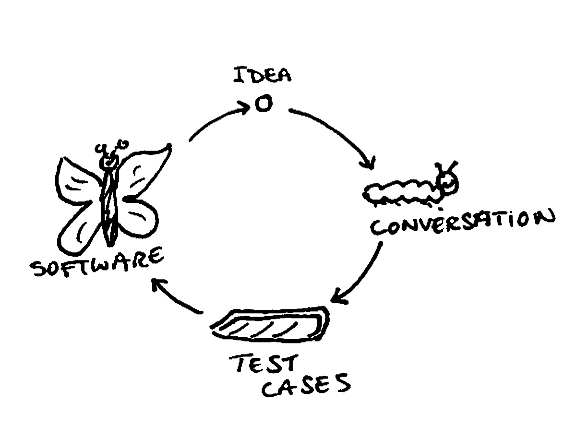
\includegraphics[width=8cm]{user_story_life_cycle}
  \caption{Ciclo de vida de uma user story}
\end{figure}

Ron Jeffries resume os aspectos críticos de uma user story como 3Cs:\\
\textbf{Cartão}: Escreva histórias nos cartões para facilitar conversas em grupos\\
\textbf{Conversa}: Faça perguntas e sugira maneiras de dividir a história\\
\textbf{Confirmação}: Chegue num acordo de como serão os testes que validarão se a história está completa\\


\section{Encorajando Conversas}
São as conversas sobre user stories que fazem com que a equipe entenda o que precisa ser feito. As conversas precisam ser guiadas pelos desenvolvedores e testadores, assegurando junto ao cliente que eles entenderam os detalhes do que precisa ser feito. Repare se a equipe está tendo problemas, e lembre-os que eles devem sempre perguntar ao cliente ao invés de chutar.

Outras conversas serão sobre as user stories futuras. Tais conversas são iniciadas pelo cliente, que não possui conhecimento técnico e precisa de uma visão do que pode ser feito no futuro.

As conversas sobre user stories não são levantadas até a reunião de planejamento. Sugira que novas user stories sejam definidas em grupos pequenos, com um cliente e alguns desenvolvedores ou testadores. Revise-as com a equipe inteira depois.


\section{Trabalhando com Cartões}
Algumas equipes fazem planejamento com um projetor sendo usado pra coletar novas user stories da equipe. Essa maneira não é tão eficiente. Uma maneira melhor de coletar user stories é usando cartões ou \textit{sticky-notes ou post-its}. É muito mais fácil agrupar user stories em cartões e movê-los pela mesa do que mover linhas e colunas numa planilha de textos.

Comece mostrando à equipe como usar os cartões. Escreva cada user story que você ouvir num cartão, e em seguida coloque-o na mesa, onde todas as pessoas possam ler. Agora todos podem contribuir com uma user story num cartão novo.

Verifique se o que você escreveu bate com o que foi dito. Caso não bata, sugira ao cliente corrigir ou reescrever o cartão. Se a história mudar, adicione notas no cartão, ou jogue-o fora e comece outro.

Não escreva todas as user stories nos cartões. Faça com que seja natural alguém sugerir uma user story e escrevê-la num cartão. Deixe cartões disponíveis no ambiente de trabalho da equipe, para que possam ser usados a qualquer momento.

Lembre-os que os cartões irão parar no quadro de tarefas e a equipe se referirá aos cartões nas daily standups. Comece com um título legível, grande e breve, no topo -- evite usar identificadores numéricos nos cartões, pois estes dificultam as conversas. É recomendável colocar estimativas no canto inferior direito em cada cartão.

\subsection{Modelo de User Story}
Para equipes que estão começando, recomenda-se usar o seguinte modelo:
``\textit{Como um}... usuário, \textit{Eu quero}... capacidade, \textit{Para que}... benefício''

Um exemplo: \textit{Como um} comprador de livros, \textit{Eu quero} ver as revisões dos compradores de um livro, \textit{Para que} eu possa decidir qual comprar.

Tal modelo ajuda a relembrar e esclarecer quem o usuário é, e qual será o benefício da história em desenvolvimento.

Essa forma de escrever user stories nem sempre é viável -- normalmente quando não há interação com usuário é difícil de expressar as intenções com este modelo.

Lembre que o propósito deste modelo de user story é ajudar a equipe a aprender a fazer perguntas que melhorem o entendimento, ao invés de preencher papéis. Uma vez que a equipe acostumar-se com user stories, descarte o modelo. Mas nunca se esqueça que o texto nos cartões devem ser entendidos por todos, sempre.

Algumas equipes preferem guardar os cartões, mesmo quando as user stories já foram implementadas e o software está funcionando, para caso precisem relembrar das histórias originais no futuro. Outras equipes jogam fora os cartões depois que a user story foi implementada.



\section{Confirmando os Detalhes}
Uma vez que a equipe entende a história, quem o usuário é, e qual problema está para ser resolvido, ela só precisa de uma maneira de discutir os detalhes do comportamento a ser implementado. Trabalhe com a equipe para criar um cojunto de testes que validam quando a user story está ``pronta''. Os testes da história\footnote{referidos por vezes como critérios de aceitação ou cenários} ajudam a equipe a esclarecer o que precisa ser feito e quanto precisa ser testado.

Os testes da história começam como pontos escritos no verso do cartão da história. Aconselhe a equipe que tais pontos são suficientes até que a história seja incluída numa iteração. Depois, esses pontos serão usados na iteração como base para criar scripts de teste.

Algumas equipes esperam que os clientes escrevam os cartões com os casos de testes em mente, mas infelizmente não é o que acontece na maioria dos casos.

Um problema está na palavra \textit{teste}. Quando ela é usada o cliente pode dar alguma desculpa pra não se envolver muito, pois o efeito que a palavra \textit{teste} tem é de parecer que se trata de algo muito técnico. Evite usar a palavra \textit{teste} com os clientes. Ao invés de pedi-los um caso de teste, peça exemplos reais de uso. Exemplos reais além de ajudarem o cliente a pensar no comportamento do software, ajudam a equipe a pensar em situações em que há necessida de manipular erros.

Comece através de uma interação de usuário simples onde um usuário alcança seu objetivo. Agora faça com que a equipe faça as seguintes perguntas ao cliente:

\begin{itemize}
\item Com que dados o usuário entra?
\item O que o usuário deve ver?
\item Há alguma regra de negócio com a qual precisamos nos preocupar?
\end{itemize}

Rascunhar a interface de usuário pode ajudar; desenhos simples são o suficiente. O interesse no momento são o conteúdo e as interações com o usuário, não na aparência.

Agora pergunte a equipe o que pode dar errado. Qual entrada de dados precisa ser tratada? Considere usar dados errados e quantidades reais. Lembre a equipe que nesse momento não é necessário trabalhar em cada condição de erro, não se trata ainda dos scripts de teste -- essa fase é exploratória.

Dan North propôs um modelo para testes de história (\textit{story test ou cenários}), que baseia-se na idéia de as pré-condições serem descritas num passo iniciado por \textit{Dado que}; as ações ficam expressas num \textit{Quando}; e o resultado da ação expresso em um \textit{Então}.\\
Por exemplo:\\
\textbf{Dado que} o usuário está visualizando a página de buscas e entra com ``Agile Coaching''\\
\textbf{Quando} o usuário clica no botão Buscar\\
\textbf{Então} são mostrado os detalhes completos do livro (título, autor, imagem do livro, sinopsis, preço, revisões) e um botão Adicionar ao Carrinho de Compras.


\begin{figure}[h]
  \centering
  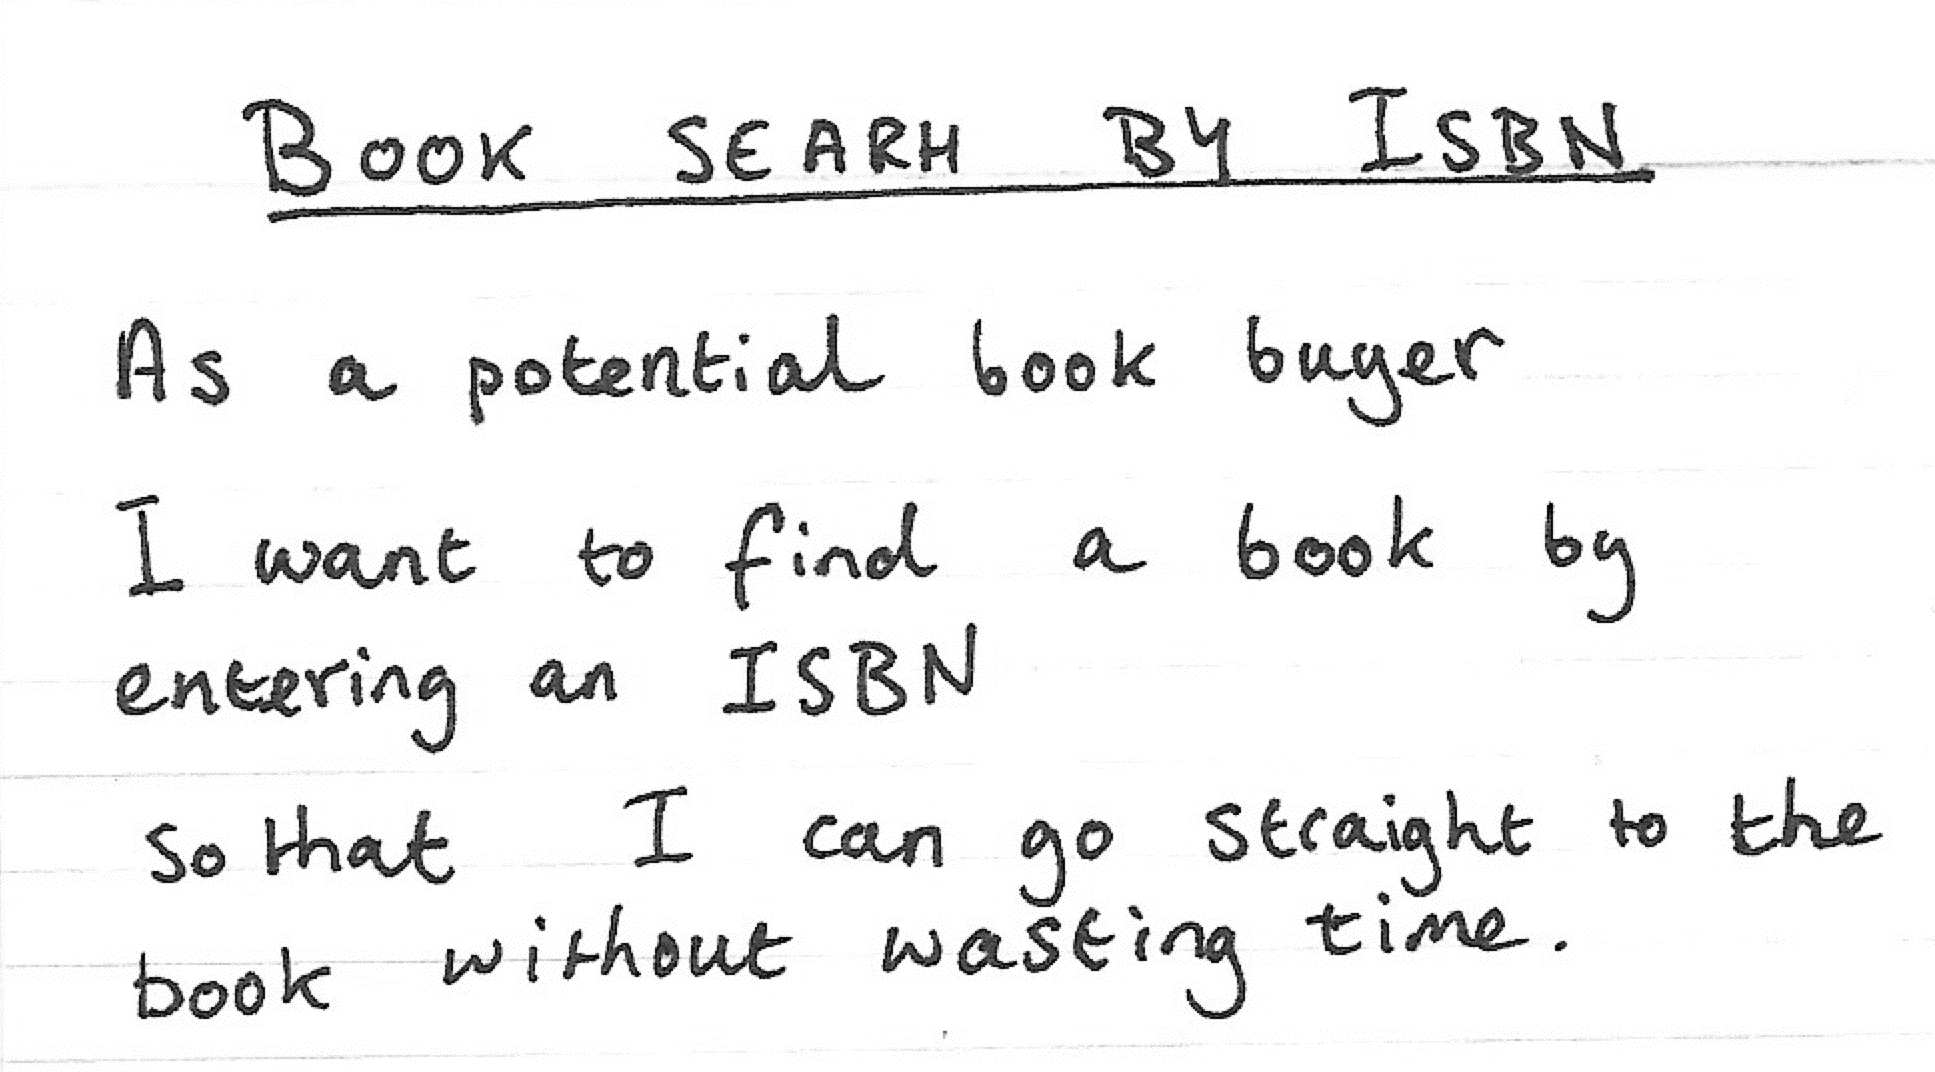
\includegraphics[width=10cm]{user_story}
  \caption{Exemplo de uma User Story}
\end{figure}

\begin{figure}[h]
  \centering
  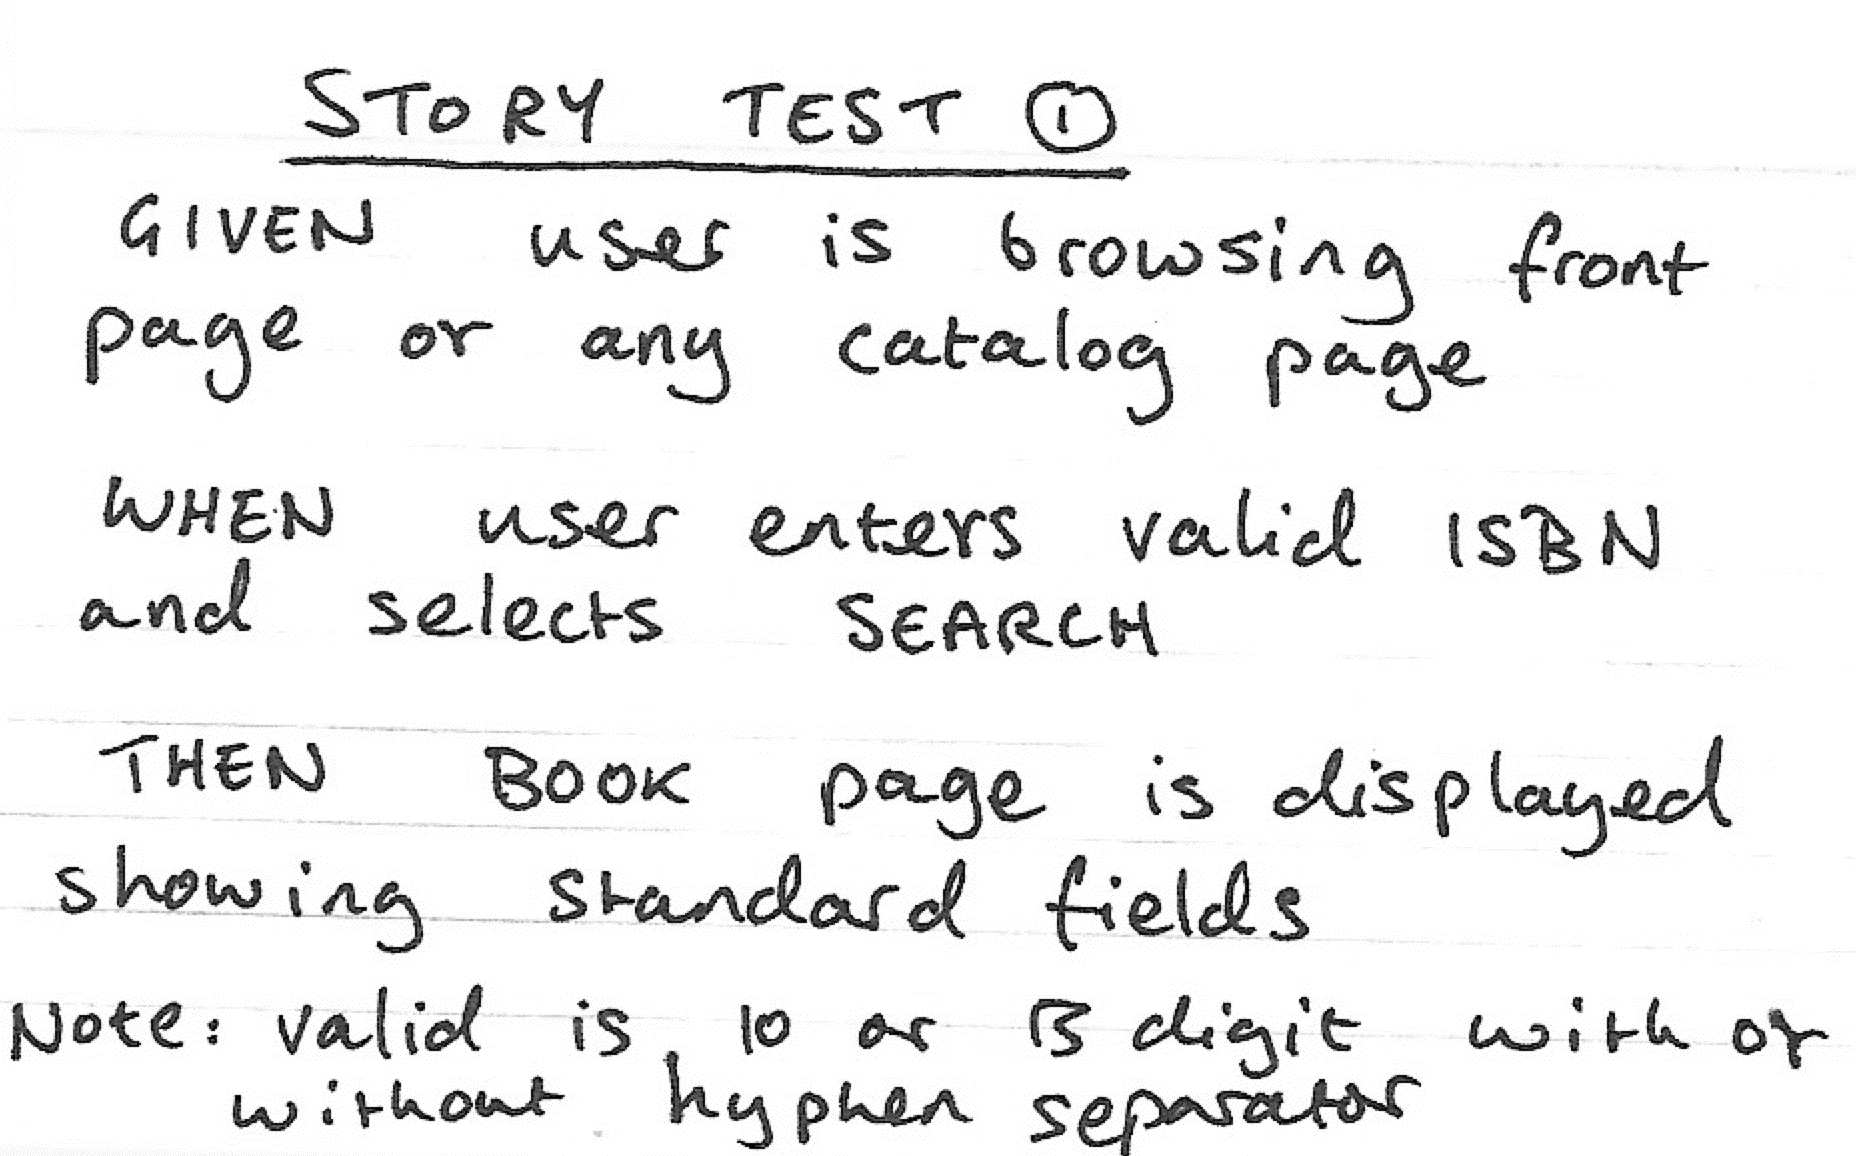
\includegraphics[width=10cm]{story_test}
  \caption{Exemplo de um teste da história (\textit{story test})}
\end{figure}


User stories são uma técnica simples que a equipe pode usar para entender melhor as intenções do cliente através de conversas sobre o que os usuários precisam. Como coach, seu foco é livrar a equipe dos mals hábitos criados na época pré-Agile. Hábitos como aceitar implementar requisitos ao pé da letra ao invés de discutir, perguntar por quês e oferecer alternativas. Ensine-os a usar os cartões, e encoraje-os a se envolver em conversas sobre user stories para oferecerem idéias e colocarem mais detalhes nos story tests.



\section{Impedimentos}

\subsection{Funcionalidade Que Não Aparece Para O Usuário}
User stories são mais eficazes quando há uma interação real do software com um usuário. Quando trata-se de user stories técnicas nem sempre há uma funcionalidade óbvia pra ser descrita\footnote{Nota do autor: veja como lidar com user stories técnicas em http://lizkeogh.com/2008/09/10/feature-injection-and-handling-technical-stories/}.


O modelo \textit{Como um...Eu quero...Para que...} não será tão útil. Mas as perguntas ``Quem quer isso? Por quê?'' ainda são relevantes para entender melhor como priorizar o trabalho. A equipe ainda deve conversar sobre o que está sendo resolvido, o benefício entregue e os testes da história que confirmarão quando a tarefa está pronta.

User stories também podem ser usadas pra agrupar tarefas técnicas que sozinhas não parecem trazer tanto benefício pro cliente -- juntas podem fazer mais sentido e usarão uma descriçao não técnica.


\subsection{Requisitos Têm Que Ser Documentados}
Algumas empresas precisam documentar requisitos formalmente, em alguns casos porque estão numa indústria regularizada e precisam usar um processo que pode ser auditado.

Você ainda pode usar user stories, mas agora será necessário documentá-las. Uma maneira rápida é criar um registro eletrônico das user stories tirando fotos ou fazendo fotocópias. Pode ser interessante fotografar os rabiscos gerados no quadro branco durante a discussão sobre a user story. Caso seja necessário uma documentação mais completa, ela pode ser escrita após a discussão sobre a user story.

Uma forma mais moderna de documentar os requisitos é automatizando-os. Os requisitos são escritos de forma executável. Ferramentas como Fit\footnote{fit.c2.com}, Cucumber\footnote{Nota do autor: http://cukes.info}, FitNesse\footnote{Nota do autor: fitnesse}, JBehave\footnote{Nota do autor: http://jbehave.org}.

\subsection{A Equipe Não Pode Estar Reunida}
Obviamente a técnica dos cartões não funciona quando a equipe está situada em diferentes localidades. User stories ainda podem servir como base de tudo nas conversas sobre as necessidades dos usuários, story tests e etc. Porém, ao invés de usar cartões (papel), você pode usar um software de área de trabalho compartilhada (\textit{Desktop sharing software}), como NetMeeting ou WebEx, para que as pessoas vejam a mesma tela. Opte por usar um software que permita escrever sticky notes virtuais.



\section{Checklist}

\begin{itemize}
\item Ensine a equipe o mantra ``Cartão, Conversa, Confirmação'' para ajudá-los a lembrar dos três elementos essenciais de uma user story. Encoraje a equipe a refinar cada user story através de conversas com o cliente.

\item Mostre à equipe como escrever histórias nos cartões escrevendo alguns.. Depois deixe que a equipe escreva os cartões sozinha.

\item Garanta que cartões ou notas estejam disponíveis no espaço de trabalho da equipe e nas reunião que discutirão histórias.

\item ``Como um... usuário Eu quero... capacidade Para que... benefício'' pode ser um modelo útil para escrever user stories. Faça com que isso não seja uma maneira de preencher papel; tais modelos devem obrigar a equipe a fazer perguntas pra si mesma. Uma vez que a equipe fizer as perguntas certas, poderá descartar o modelo.

\item Ajude o cliente a trabalhar nos detalhes das histórias antes das sessões de planejamento. Uma maneira de começar a dar forma às user stories é envolvendo poucos membros da equipe antes da sessão; eles podem fazer pergutas e sugerir story tests.

\end{itemize}








\end{document}

